% Options for packages loaded elsewhere
\PassOptionsToPackage{unicode}{hyperref}
\PassOptionsToPackage{hyphens}{url}
\PassOptionsToPackage{dvipsnames,svgnames,x11names}{xcolor}
%
\documentclass[
  authoryear,
  preprint,
  1p]{elsarticle}

\usepackage{amsmath,amssymb}
\usepackage{iftex}
\ifPDFTeX
  \usepackage[T1]{fontenc}
  \usepackage[utf8]{inputenc}
  \usepackage{textcomp} % provide euro and other symbols
\else % if luatex or xetex
  \usepackage{unicode-math}
  \defaultfontfeatures{Scale=MatchLowercase}
  \defaultfontfeatures[\rmfamily]{Ligatures=TeX,Scale=1}
\fi
\usepackage{lmodern}
\ifPDFTeX\else  
    % xetex/luatex font selection
\fi
% Use upquote if available, for straight quotes in verbatim environments
\IfFileExists{upquote.sty}{\usepackage{upquote}}{}
\IfFileExists{microtype.sty}{% use microtype if available
  \usepackage[]{microtype}
  \UseMicrotypeSet[protrusion]{basicmath} % disable protrusion for tt fonts
}{}
\makeatletter
\@ifundefined{KOMAClassName}{% if non-KOMA class
  \IfFileExists{parskip.sty}{%
    \usepackage{parskip}
  }{% else
    \setlength{\parindent}{0pt}
    \setlength{\parskip}{6pt plus 2pt minus 1pt}}
}{% if KOMA class
  \KOMAoptions{parskip=half}}
\makeatother
\usepackage{xcolor}
\setlength{\emergencystretch}{3em} % prevent overfull lines
\setcounter{secnumdepth}{5}
% Make \paragraph and \subparagraph free-standing
\ifx\paragraph\undefined\else
  \let\oldparagraph\paragraph
  \renewcommand{\paragraph}[1]{\oldparagraph{#1}\mbox{}}
\fi
\ifx\subparagraph\undefined\else
  \let\oldsubparagraph\subparagraph
  \renewcommand{\subparagraph}[1]{\oldsubparagraph{#1}\mbox{}}
\fi


\providecommand{\tightlist}{%
  \setlength{\itemsep}{0pt}\setlength{\parskip}{0pt}}\usepackage{longtable,booktabs,array}
\usepackage{calc} % for calculating minipage widths
% Correct order of tables after \paragraph or \subparagraph
\usepackage{etoolbox}
\makeatletter
\patchcmd\longtable{\par}{\if@noskipsec\mbox{}\fi\par}{}{}
\makeatother
% Allow footnotes in longtable head/foot
\IfFileExists{footnotehyper.sty}{\usepackage{footnotehyper}}{\usepackage{footnote}}
\makesavenoteenv{longtable}
\usepackage{graphicx}
\makeatletter
\def\maxwidth{\ifdim\Gin@nat@width>\linewidth\linewidth\else\Gin@nat@width\fi}
\def\maxheight{\ifdim\Gin@nat@height>\textheight\textheight\else\Gin@nat@height\fi}
\makeatother
% Scale images if necessary, so that they will not overflow the page
% margins by default, and it is still possible to overwrite the defaults
% using explicit options in \includegraphics[width, height, ...]{}
\setkeys{Gin}{width=\maxwidth,height=\maxheight,keepaspectratio}
% Set default figure placement to htbp
\makeatletter
\def\fps@figure{htbp}
\makeatother

\makeatletter
\@ifpackageloaded{caption}{}{\usepackage{caption}}
\AtBeginDocument{%
\ifdefined\contentsname
  \renewcommand*\contentsname{Table of contents}
\else
  \newcommand\contentsname{Table of contents}
\fi
\ifdefined\listfigurename
  \renewcommand*\listfigurename{List of Figures}
\else
  \newcommand\listfigurename{List of Figures}
\fi
\ifdefined\listtablename
  \renewcommand*\listtablename{List of Tables}
\else
  \newcommand\listtablename{List of Tables}
\fi
\ifdefined\figurename
  \renewcommand*\figurename{Figure}
\else
  \newcommand\figurename{Figure}
\fi
\ifdefined\tablename
  \renewcommand*\tablename{Table}
\else
  \newcommand\tablename{Table}
\fi
}
\@ifpackageloaded{float}{}{\usepackage{float}}
\floatstyle{ruled}
\@ifundefined{c@chapter}{\newfloat{codelisting}{h}{lop}}{\newfloat{codelisting}{h}{lop}[chapter]}
\floatname{codelisting}{Listing}
\newcommand*\listoflistings{\listof{codelisting}{List of Listings}}
\makeatother
\makeatletter
\makeatother
\makeatletter
\@ifpackageloaded{caption}{}{\usepackage{caption}}
\@ifpackageloaded{subcaption}{}{\usepackage{subcaption}}
\makeatother
\journal{Behavior Research Methods}
\ifLuaTeX
  \usepackage{selnolig}  % disable illegal ligatures
\fi
\usepackage[]{natbib}
\bibliographystyle{elsarticle-harv}
\usepackage{bookmark}

\IfFileExists{xurl.sty}{\usepackage{xurl}}{} % add URL line breaks if available
\urlstyle{same} % disable monospaced font for URLs
\hypersetup{
  pdftitle={Everything, altogether, all at once: addressing data challenges when measuring speech intelligibility through entropy scores},
  pdfauthor={Jose Manuel Rivera Espejo; Sven De Maeyer; Steven Gillis},
  pdfkeywords={Bayesian analysis, speech intelligibility, bounded
outcomes, clustering, measurement
error, outliers, heteroscedasticity, generalized linear latent and mixed
models, robust regression models.},
  colorlinks=true,
  linkcolor={blue},
  filecolor={Maroon},
  citecolor={Blue},
  urlcolor={Blue},
  pdfcreator={LaTeX via pandoc}}

\setlength{\parindent}{6pt}
\begin{document}

\begin{frontmatter}
\title{Everything, altogether, all at once: addressing data challenges
when measuring speech intelligibility through entropy scores}
\author[1]{Jose Manuel Rivera Espejo%
\corref{cor1}%
}
 \ead{JoseManuel.RiveraEspejo@uantwerpen.be} 
\author[1]{Sven De Maeyer%
%
}
 \ead{sven.demaeyer@uantwerpen.be} 
\author[2]{Steven Gillis%
%
}
 \ead{steven.gillis@uantwerpen.be} 

\affiliation[1]{organization={University of Antwerp, Department of
Training and Education Sciences},,postcodesep={}}
\affiliation[2]{organization={University of Antwerp, Department of
Linguistics},,postcodesep={}}

\cortext[cor1]{Corresponding author}



        
\begin{abstract}
Considering the imperative need to comprehensively address all data
features when investigating unobservable and complex traits, this
research aims to showcase the effectiveness of the Generalized Linear
Latent and Mixed Model (GLLAMM)
\citep{Rabe_et_al_2004a, Rabe_et_al_2004b, Rabe_et_al_2004c, Skrondal_et_al_2004a}
in handling entropy scores for investigating speech intelligibility
theories. Utilizing transcriptions from spontaneous speech data
originally collected by \citet{Boonen_et_al_2021}, the Bayesian
Beta-proportion GLLAMM was employed to model the resulting entropy
scores. The study compared the model's prediction accuracy with the
Normal Linear Mixed Model (LMM) \citep{Holmes_et_al_2019} and
investigated its capacity to estimate a latent intelligibility from
manifest entropy scores. Additionally, it illustrated how the model can
explore research theories concerning the impact of speaker-related
factors on intelligibility. Results demonstrate the consistent
superiority of the Beta-proportion GLLAMM over the Normal LMM in
predicting the empirical phenomena. Furthermore, the model effectively
quantified the latent potential intelligibility, enabling the ranking
and comparison of individuals while accommodating for uncertainties.
Lastly, it facilitated exploration of theories related to
speaker-related factors and intelligibility. Despite these advantages,
the introduction of these innovative statistical tools poses challenges
for researchers seeking implementation. Nevertheless, the study suggests
interesting future research directions, including power analysis, causal
hypothesis formulation, and exploration of novel methods for
intelligibility assessment. This study has implications for researchers
and data analysts interested in quantitatively measuring and testing
theories related to intricate, unobservable constructs, while
emphasizing the accurate prediction of empirical phenomena.
\end{abstract}





\begin{keyword}
    Bayesian analysis \sep speech intelligibility \sep bounded
outcomes \sep clustering \sep measurement
error \sep outliers \sep heteroscedasticity \sep generalized linear
latent and mixed models \sep 
    robust regression models.
\end{keyword}
\end{frontmatter}
    
\section{Introduction}\label{sec-introduction}

Intelligibility is at the core of successful, felicitous communication.
Thus, being able to speak intelligibly is a major achievement in
language acquisition and development. Moreover, intelligibility is
considered to be the most practical index to assess competence in oral
communication \citep{Kent_et_al_1994}. Consequently, it serves as a key
indicator for evaluating the effectiveness of various interventions like
speech therapy or cochlear implantation \citep{Chin_et_al_2012}.

The notion of speech intelligibility may appear deceptively simple, yet
it is an intricate concept filled with inherent challenges in its
assessment. Intelligibility refers to the extent to which a listener can
accurately recover the elements in a speaker's acoustic signal, such as
phonemes or words
\citep{Freeman_et_al_2017, vanHeuven_2008, Whitehill_et_al_2004}.
Furthermore, achieving intelligible spoken language requires all core
components of speech perception, cognitive processing, linguistic
knowledge, and articulation to be mastered \citep{Freeman_et_al_2017}.
Hence, it is unsurprising that its accurate measurement faces challenges
\citep{Kent_et_al_1989}. These challenges arise from the interplay of
its determinants, which encompass attributes of the communicative
environment, such as background noise \citep{Munro_1998}, speaker
features like speaking rate \citep{Munro_et_al_1998} or accent
\citep{Jenkins_2000, Ockey_et_al_2016}, and listener characteristics
like vocabulary proficiency or hearing ability
\citep{Varonis_et_al_1985}.

While several approaches have been proposed to assess intelligibility,
they commonly rely on two types of speech samples: read-aloud or
imitated, and spontaneous speech samples. Most studies favor read-aloud
or imitated speech samples due to the substantial control they offer in
selecting stimuli for intelligibility assessment. Additionally, these
types of speech facilitate a direct and unambiguous comparison between a
defined word target, produced by a speaker, and the listener's
identification of it, as exemplified by multiple studies such as
\citet{Castellanos_et_al_2014}, \citet{Chin_et_al_2012},
\citet{Chin_et_al_2014}, \citet{Freeman_et_al_2017},
\citet{Khwaileh_et_al_2010}, and \citet{Montag_et_al_2014}. However, it
has been demonstrated that these controlled speech samples exhibit
limited efficacy in predicting intelligibility among hearing-impaired
individuals \citep{Cox_et_al_1989, Ertmer_2011}. \textcolor{blue}{In contrast,
spontaneous speech samples offer a more ecologically valid approach to
assess intelligibility, resembling everyday informal speech more than
read-aloud or imitated speech samples \citep{Boonen_et_al_2021}.
However, due to the significant uncertainty surrounding the speaker's
intended word production, it is time-consuming or straight unfeasible to
establish a word target for these samples
\citep{Flipsen_2006, Lagerberg_et_al_2014}. This renders conventional
accuracy metrics from imitated speech, such as the percentage of read or
imitated words, impractical \citep{Boonen_et_al_2021}.}

\textcolor{blue}{Yet, various metrics of intelligibility can still be derived from
transcriptions of spontaneous speech samples, including the percentage
of (un)intelligible words or syllables
\citep{Flipsen_2006, Lagerberg_et_al_2014}, as well as entropy scores
\citep{Boonen_et_al_2021}. In the latter approach, listeners transcribe
orthographically multiple spontaneous speech samples produced by various
speakers.} These transcriptions are then aggregated into entropy scores,
where lower scores indicate a higher degree of agreement among the
listener's transcriptions and, consequently, higher intelligibility,
while higher scores suggest lower intelligibility due to a lower degree
of agreement in the transcriptions
\citep{Boonen_et_al_2021, Faes_et_al_2022}. Notably, the aggregation
procedure assumes that speech samples are considered `intelligible' if
all listeners decode them in the same manner. These scores have been
instrumental in examining differences in speakers' speech
intelligibility, particularly between children with normal hearing and
those with cochlear implants \citep{Boonen_et_al_2021}.

However, despite their potential as a fine-grained metric of
intelligibility, as proposed by \citet{Boonen_et_al_2021}, they exhibit
a statistical complexity that cautions researchers against treating them
as straightforward indices of intelligibility. This complexity emerges
from the processes of data collection and transcription aggregation,
endowing the scores with four distinctive features: boundedness,
measurement error, clustering, and the possible presence of outliers and
heteroscedasticity. Firstly, entropy scores are confined to the interval
between zero and one, a phenomenon known as boundedness. Boundedness
refers to the restriction of data values within specific bounds or
intervals, beyond which they cannot occur \citep{Lebl_2022}. \textcolor{blue}{Secondly,
entropy scores are assumed to be a manifestation of a speaker's
intelligibility, with this intelligibility being the primary factor
influencing the observed scores.} This issue is commonly referred to as
measurement error, signifying the disparity between the observed values
of a variable, recorded under similar conditions, and some fixed
\emph{true value} which is not directly observable
\citep{Everitt_et_al_2010}. Thirdly, due to the repeated assessment of
speakers through multiple speech samples, the scores exhibit clustering.
Clustering occurs when outcomes stem from repeated measurements of the
same individual, location, or time \citep{McElreath_2020}. \textcolor{blue}{Lastly,
driven by speech samples with entropy scores located at the extreme of
the bounds, and the existence of more than one population in the data
under scrutiny (i.e., normal hearing versus hearing-impaired speakers),
the scores may exhibit a potential for outliers and heteroscedasticity.
Outliers are observations that markedly deviate from other sample data
points where they occur \citep{Grubbs_1969}, while heteroscedasticity
occurs when the outcome's variance depends on the values of another
variable \citep{Everitt_et_al_2010}.}

Failure to collectively address these data features can result in
numerous statistical challenges that might hamper the researcher's
ability to investigate intelligibility. Notably, neglecting boundedness
can, at best, lead to underfitting and, at worst, to misspecification.
Underfitting occurs when statistical models fail to capture the
underlying data patterns, potentially causing the generation of
predictions outside the data range, thus hindering the model's ability
to generalize when confronted with new data. Conversely,
misspecification, marked by a poor representation of relevant aspects of
the true data in the model's functional form, can lead to inconsistent
and less precise parameter estimates \citep{Everitt_et_al_2010}.
Additionally, overlooking issues such as measurement error, clustering,
outliers, or heteroscedasticity can lead to biased and less precise
parameter estimates \citep{McElreath_2020}, ultimately diminishing the
statistical power of models and increasing the likelihood of committing
type I or type II errors when addressing research inquiries.

In the realm of computational statistics and data analysis, several
models have been developed to address some of these data features
individually and, at times, collectively. For instance,
\citet{Ferrari_et_al_2004} and \citet{Simas_et_al_2010} initially
introduced and expanded beta regression models to handle outcomes
constrained within the unit interval. Subsequently,
\citet{Figueroa-Zuniga_et_al_2013} extended these models to address data
clustering. Over time, beta regression models have evolved to
accommodate clustering and measurement errors in covariates, as
demonstrated by \citet{Carrasco_et_al_2012} and
\citet{Figueroa-Zuniga_et_al_2018}. Furthermore, robust versions of
these models have been proposed to account for other statistical data
issues, such as outliers and heteroscedasticity, as seen in
\citet{Bayes_et_al_2012} and \citet{Figueroa-Zuniga_et_al_2021}. Robust
models are a general class of statistical procedures designed to reduce
the sensitivity of the parameter estimates to mild or moderate
departures of the data from the model's assumptions
\citep{Everitt_et_al_2010}. Ultimately, the work of Rabe-Hesketh and
colleagues introduced the Generalized Linear Latent and Mixed Model
(GLLAMM)
\citep{Rabe_et_al_2004a, Rabe_et_al_2004b, Rabe_et_al_2004c, Skrondal_et_al_2004a},
a unified framework that can simultaneously tackle with all of the
aforementioned data features.

All of these models have found moderate adoption in various fields,
including speech communication \citep{Boonen_et_al_2021}, psychology
\citep{Unlu_et_al_2017}, cognition
\citep{Verkuilen_et_al_2012, Lopes_et_al_2023}, education
\citep{Pereira_et_al_2020}, health care
\citep{Ghosh_2019, Kangmennaang_et_al_2023}, chemistry
\citep{de_Brito_et_al_2021}, and policy analysis
\citep{Dieteren_et_al_2023, Choi_2023, Zhang_et_al_2023}. Specifically,
in the domain of speech communication, \citet{Boonen_et_al_2021}
addressed data clustering within the context of intelligibility
research. Conversely, \citet{de_Brito_et_al_2021} and
\citet{Kangmennaang_et_al_2023} concentrated on tackling non-normal
bounded data with measurement error in covariates, within the context of
chemical reactions and health care access, respectively. Remarkably,
despite these individual efforts, there is, to the best of the authors'
knowledge, no study comprehensively addressing all of these data
features in a principled way, while also transparently and
systematically documenting the Bayesian estimation of the resulting
statistical models.

\textcolor{blue}{The study employed Bayesian procedures due to three primary properties.
Firstly, prior research consistently shows that Bayesian methods
outperforms frequentist methods when handling complex and
over-parameterized models \citep{Baker_1998, Kim_et_al_1999}. This
property is particularly relevant when dealing with the proposed
Generalized Linear Latent and Mixed Models (GLLAMM), which may be
challenging to program or may not be viable under frequentist methods
\citep{Depaoli_2014}. Secondly, the Bayesian approach enables the
incorporation of prior information, thereby constraining certain
parameters within specified bounds. This feature helps address issues
such as non-convergence or improper parameter estimation commonly
encountered in complex models under frequentist methods
\citep{Martin_et_al_1975, Seaman_et_al_2011}. An example of this issue
is the estimation of negative variances for random effects in
hierarchical models \citep{Holmes_et_al_2019}, which this study resolves
by utilizing prior distributions. Lastly, Bayesian methods have shown
proficiency in handling relatively small sample sizes
\citep{Baldwin_et_al_2013, Lambert_et_al_2005, Depaoli_2014}. Although
this study models 2,263 entropy scores, they are derived from a modest
sample size of 32 speakers, from which inferences are drawn.
Consequently, relying solely on the asymptotic properties of frequentist
methods may not be justified in this context, highlighting the relevance
of this property for the study.}

\subsection{Research questions}\label{sec-I-RQ}

Considering the imperative need to comprehensively address all data
features when investigating unobservable and complex traits, this
investigation aims to demonstrate the efficacy of the Generalized Linear
Latent and Mixed Model (GLLAMM) in handling entropy scores features when
exploring research theories concerning speech intelligibility. To
achieve this objective, the study will reexamine data originating from
transcriptions of spontaneous speech samples, initially collected by
\citet{Boonen_et_al_2021}. Subsequently, this data will be aggregated
into entropy scores and subjected to modeling through the Bayesian
Beta-proportion GLLAMM.

To address the primary objective, the study poses three key research
questions. First, given the importance of accurate predictions in
developing useful practical models and testing research theories
\citep{Shmueli_et_al_2012}, \emph{Research Question 1 (RQ1)} evaluates
whether the Beta-proportion GLLAMM yields more accurate predictions than
the widely used Normal Linear Mixed Model (LMM)
\citep{Holmes_et_al_2019}. Second, acknowledging that intelligibility is
an unobservable, intricate concept and a key indicator of oral
communication competence \citep{Kent_et_al_1994}, \emph{Research
Question 2 (RQ2)} investigates how the proposed model can estimate
speakers' latent intelligibility from manifest entropy scores. Thirdly,
recognizing that research involves developing and comparing theories,
\emph{Research Question 3 (RQ3)} illustrates how these research theories
can be examined within the model's framework. Specifically, RQ3 assesses
the influence of speaker-related factors on the newly estimated latent
intelligibility.

\textcolor{blue}{Ultimately, this study offers a statistical tool that improves upon
current research models for researchers studying speech intelligibility
through entropy scores and those in similar or different fields facing
analogous data challenges. This tool assess the predictability of
empirical phenomena and develops a quantitative measure for the latent
variable of interest. This quantitative measure, in turn, facilitates
the appropriate comparison of existing theories related to the latent
variable, and even encourages the formulation of new ones.}

\section{Methods}\label{sec-methods}

\subsection{Data}\label{sec-M-D}

The data comprised the transcriptions of spontaneous speech samples
originally collected by \citet{Boonen_et_al_2021}. The data is not
publicly available due to privacy restrictions. Nonetheless, the data
can be provided by the corresponding author upon reasonable request.

\subsubsection{Speakers}\label{sec-M-S}

\citet{Boonen_et_al_2021} selected \(32\) speakers, comprising \(16\)
normal hearing children (NH) and \(16\) hearing-impaired children with
cochlear implants (HI/CI). At the time of the collection of the speech
samples, the NH group were between \(68\) and \(104\) months old
(\(M=86.3\), \(SD=9.0\)), while HI/CI group were between \(78\) and
\(98\) months old (\(M=86.3\), \(SD=6.7\)). \textcolor{blue}{All children were native
speakers of Belgian Dutch.}

\subsubsection{Speech samples}\label{sec-M-SS}

Boonen and colleagues selected speech samples from a large corpus of
children's spontaneously spoken speech recordings. \textcolor{blue}{These recordings
were made in Belgian Dutch and obtained while the children narrated a
story prompted by the picture book ``Frog, Where Are You?''
\citep{Mayer_1969} to a caregiver `unfamiliar with the story'.} Before
recording, the children were allowed to skim over the booklet and
examine pictures. Prior to the selection process, the recordings were
orthographically transcribed using the CHAT format in the CLAN editor
\citep{MacWhinney_2020}. These transcriptions were exclusively used in
the curation of appropriate speech samples. To ensure the quality of the
selection, Boonen and colleagues excluded sentences containing
syntactically ill-formed or incomplete statements, with background
noise, crosstalk, long hesitations, revisions, or non-words. Finally,
ten speech samples were randomly chosen for each of the \(32\) selected
speakers. Each of these samples comprised a single sentence with a
length of three to eleven words (\(M=7.1\), \(SD=1.1\)). The process
resulted in a total of \(320\) selected sentences collectively
comprising \(2,263\) words.

\subsubsection{Listeners}\label{sec-M-L}

Boonen and colleagues recruited \(105\) students from the University of
Antwerp. All participants were native speakers of Belgian Dutch and
reported no history of hearing difficulties or prior exposure to the
speech of hearing-impaired speakers.

\subsubsection{Transcription task and entropy scores}\label{sec-M-TS}

\textcolor{blue}{\citet{Boonen_et_al_2021} distributed the \(320\) speech samples and
\(105\) listeners into five blocks through random allocation. Each block
comprised \(21\) listeners and \(64\) sentences. The listeners were
tasked with transcribing each sentence, which were presented to them in
a random order. This resulted in a total of \(47,514\) transcribed words
from the original \(2,263\) words available in the speech samples. These
orthographic transcriptions were automatically aligned with a python
script \citep{Boonen_et_al_2021}, at the sentence level in a column-like
grid structure like the one presented in Table~\ref{tbl-alignment}.}
This alignment process was repeated for each sentence within each
speaker and block, and the output was manually checked and adjusted (if
needed) in order to appropriately align the words. \textcolor{blue}{For more details on
the random assignment and alignment procedures refer to the
aforementioned authors.}

Next, this study aggregated the aligned transcriptions by listener
yielding \(2,2634\) entropy scores, one score per word. The entropy
scores were calculated following Shannon's formula
\citeyearpar{Shannon_1948}:

\begin{equation}\phantomsection\label{eq-entropy}{
H_{wsib} = \frac{ -\left[ \sum_{k=1}^{K}  p_{k} \cdot log_{2}(p_{k}) \right] }{ log_{2}(J)}
}\end{equation}

where \(H_{wsib}\) denotes the entropy scores confined to an interval
between zero and one, with \(w\) defining the word index, \(s\) the
sentence index, \(i\) the speaker index, and \(b\) the block index.
Moreover, \(K\) describes the number of different word types within
transcriptions, and \(J\) defines the total number of word
transcriptions. Notice that by design, the total number of word
transcriptions \(J\) corresponds with the number of listeners per block,
i.e., \(21\) listeners. Lastly, \(p_{k} = \sum_{j=1}^{J} 1(T_{jk}) / J\)
denotes the proportion of word types within transcriptions, with
\(1(T_{jk})\) describing an indicator function that takes the value of
one when the word type \(k\) is present in the transcription \(j\). See
Section~\ref{sec-appA} for a calculation example of entropy scores.

These entropy scores served as the outcome variable, capturing agreement
or disagreement among listeners' word transcriptions. Lower scores
indicated a higher degree of agreement between transcriptions and
therefore higher intelligibility, while higher scores indicated lower
intelligibility, due to a lower degree of agreement in the
transcriptions \citep{Boonen_et_al_2021, Faes_et_al_2022}. Furthermore,
no score is excluded from the modeling process using univariate
procedures, rather, the identification of highly influential
observations is performed within the context of the proposed models, as
recommended by \citet{McElreath_2020}.

\begin{longtable}[]{@{}
  >{\centering\arraybackslash}p{(\columnwidth - 10\tabcolsep) * \real{0.2222}}
  >{\centering\arraybackslash}p{(\columnwidth - 10\tabcolsep) * \real{0.1389}}
  >{\centering\arraybackslash}p{(\columnwidth - 10\tabcolsep) * \real{0.1389}}
  >{\centering\arraybackslash}p{(\columnwidth - 10\tabcolsep) * \real{0.1389}}
  >{\centering\arraybackslash}p{(\columnwidth - 10\tabcolsep) * \real{0.1389}}
  >{\centering\arraybackslash}p{(\columnwidth - 10\tabcolsep) * \real{0.1389}}@{}}
\caption{Hypothetical alignment of word transcriptions and entropy
scores. \textbf{\emph{Note:}} Extracted from Boonen et al.
\citeyearpar{Boonen_et_al_2021}, and slightly modified for illustrative
purposes. Entropy scores are calculated the first sentence, produced by
the first speaker assigned to the first block, and transcribed by five
listeners \(\left( s=1, i=1, b=1, J=5 \right)\). Transcriptions are in
Belgian Dutch followed by their English translation. \emph{{[}B{]}}
represent a blank space, and \emph{{[}X{]}} an unidentifiable
speech.}\label{tbl-alignment}\tabularnewline
\toprule\noalign{}
\begin{minipage}[b]{\linewidth}\centering
Transcription
\end{minipage} & \begin{minipage}[b]{0.7\textwidth}\centering
Words
\end{minipage} & \begin{minipage}[b]{\linewidth}\centering
\end{minipage} & \begin{minipage}[b]{\linewidth}\centering
\end{minipage} & \begin{minipage}[b]{\linewidth}\centering
\end{minipage} & \begin{minipage}[b]{\linewidth}\centering
\end{minipage} \\
\begin{minipage}[b]{\linewidth}\centering
Number
\end{minipage} & \begin{minipage}[b]{\linewidth}\centering
1
\end{minipage} & \begin{minipage}[b]{\linewidth}\centering
2
\end{minipage} & \begin{minipage}[b]{\linewidth}\centering
3
\end{minipage} & \begin{minipage}[b]{\linewidth}\centering
4
\end{minipage} & \begin{minipage}[b]{\linewidth}\centering
5
\end{minipage} \\
\midrule\noalign{}
\endfirsthead
\toprule\noalign{}
\endlastfoot
1 & de & jongen & ziet & een & kikker \\
& the & boy & sees & a & frog \\
2 & de & jongen & ziet & de & {[}X{]} \\
& the & boy & sees & the & {[}X{]} \\
3 & de & jongen & zag & {[}B{]} & kokkin \\
& the & boy & saw & {[}B{]} & cook \\
4 & de & jongen & zag & geen & kikkers \\
& the & boy & saw & no & frogs \\
5 & de & hond & zoekt & een & {[}X{]} \\
& the & dog & searches & a & {[}X{]} \\
\textbf{Entropy} & \(0\) & \(0.3109\) & \(0.6555\) & \(0.8277\) &
\(1\) \\
\end{longtable}

\subsection{Statistical models}\label{sec-M-SM}

This section articulates the probabilistic formalism of both the Normal
LMM and the proposed Beta-proportion GLLAMM. Subsequently, it details
the set of fitted models and the estimation procedure, along with the
criteria employed to assess the quality of the Bayesian inference
results. Lastly, the section outlines the methodology employed for model
comparison.

\subsubsection{Normal LMM}\label{sec-M-SM-NLMM}

The general mathematical formalism of the Normal LMM posits that the
likelihood of the (manifest) entropy scores follow a normal
distribution, i.e.

\begin{equation}\phantomsection\label{eq-normal-LMM-likelihood}{
H_{wsib} \sim \text{Normal} \left( \mu_{sib}, \sigma_{i} \right)
}\end{equation}

where \(\mu_{sib}\) represents the average entropy at the word-level and
\(\sigma_{i}\) denotes the standard deviation of the average entropy at
the word-level, varying for each speaker. Given the clustered nature of
the data, \(\mu_{sib}\) is defined by the linear combination of
individual characteristics and several random effects:

\begin{equation}\phantomsection\label{eq-normal-LMM-linearpred}{
\mu_{sib} = \alpha + \alpha_{HS[i]} + \beta_{A, HS[i]} (A_{i} - \bar{A}) + u_{si} + e_{i} + a_{b}
}\end{equation}

where \(HS_{i}\) and \(A_{i}\) denote the hearing status and
chronological age of speaker \(i\), respectively. Additionally,
\(\alpha\) denote the general intercept, \(\alpha_{HS[i]}\) represents
the average entropy for each hearing status group, and
\(\beta_{A,HS[i]}\) denotes the evolution of the average entropy per
unit of chronological age \(A_{i}\) for each hearing status group.
Furthermore, \(u_{si}\) denotes the sentence-speaker random effects
measuring the unexplained entropy variability within sentences for each
speaker, \(e_{i}\) denotes the speaker random effects describing the
unexplained entropy variability between speakers, and \(a_{b}\) denotes
the block random effects assessing the unexplained variability between
experimental blocks.

Several notable features of the Normal LLM can be discerned from the
equations. Firstly, Equation~\ref{eq-normal-LMM-likelihood} indicates
that the variability of the average entropy at the word level can differ
for each speaker, enhancing the model \emph{robustness} to mild or
moderate data departures from the normal distribution assumption, such
as in the presence of heteroscedasticity or outliers. \textcolor{blue}{Secondly,
Equation~\ref{eq-normal-LMM-linearpred} reveals that the model assumes
no transformation is applied to the relationship between the average
entropy and the linear combination of speakers' characteristics. This is
commonly known as a direct link function. Moreover, the equation
indicates that chronological age is \emph{centered} around the minimum
chronological age in the sample \(\bar{A}\). The \emph{centering}
procedure prevents the interpretation of parameters outside the range of
chronological ages available in the data \citep{Everitt_et_al_2010}.
Additionally, the equation implies the model considers separate
intercept and separate age slopes for each hearing status group, i.e.,
\(\alpha_{HS[i]}\) and \(\beta_{A, HS[i]}\) for NH and HI/CI speakers,
respectively. Finally, the presence of a general intercept \(\alpha\) in
the equation reveals that the model is over-parameterized. Although the
estimation of over-parameterized models is only possible under Bayesian
methods, their estimation does not violate any statistical principle
\citep[pp.~345]{McElreath_2020}. In contrast, this over-parameterized
model facilitated: (1) the comparison between the specific parameter
interpretations of the Normal LMM and the Beta-proportion GLLAMM, with
\(\alpha\) serving no particular purpose, and (2) the assignment of
prior distributions.}

\subsubsection{Beta-proportion GLLAMM}\label{sec-M-SM-BGLLAMM}

The general mathematical formalism of the proposed Beta-proportion
GLLAMM comprises four components: a response model likelihood, a linear
predictor, a link function, and a structural model. The likelihood of
response model posits the entropy scores follow a Beta-proportion
distribution,

\begin{equation}\phantomsection\label{eq-beta-GLLAMM-likelihood}{
H_{wsib} \sim \text{BetaProp} \left( \mu_{ib}, M_{i} \right)
}\end{equation}

where\(\mu_{ib}\) denotes the average entropy at the word-level and
\(M_{i}\) signifies the \emph{dispersion} of the average entropy at the
word-level, varying for each speaker. Additionally, \(\mu_{ib}\) is
defined as,

\begin{equation}\phantomsection\label{eq-beta-GLLAMM-linpred}{
\mu_{ib} = \text{logit}^{-1}[ a_{b} - SI_{i} ]
}\end{equation}

where \(\text{logit}^{-1}(x) = exp(x) / (1+exp(x))\) is the
inverse-logit link function, \(a_{b}\) denotes the block random effects,
and \(SI_{i}\) describes the speaker's latent \emph{potential
intelligibility}. Conversely, the structural equation model relates the
speakers' latent potential intelligibility to the individual
characteristics:

\begin{equation}\phantomsection\label{eq-beta-GLLAMM-structural}{
SI_{i} = \alpha + \alpha_{HS[i]} + \beta_{A, HS[i]} (A_{i} - \bar{A}) + e_{i} + u_{i}
}\end{equation}

where \(\alpha\) defines the general intercept, \(\alpha_{HS[i]}\)
denotes the potential intelligibility for different hearing status
groups, and \(\beta_{A,HS[i]}\) indicates the evolution of potential
intelligibility per unit of chronological age for each hearing status
group. Furthermore, \(e_{i}\) represents speakers block effects,
describing unexplained potential intelligibility variability between
speakers, and \(u_{i} = \sum_{s=1}^{S} u_{si}/S\) denotes sentence
random effects, assessing the average unexplained potential
intelligibility variability among sentences within each speaker, with
\(S\) denoting the total number of sentences per speaker.

Several features are evident in this probabilistic representation.
Firstly, akin to the Normal LMM,
Equation~\ref{eq-beta-GLLAMM-likelihood} reveals that the
\emph{dispersion} of average entropy at the word level can differ for
each speaker. This enhances the model's robustness to mild or moderate
data departures from the beta-proportion distribution assumption.
Secondly, in contrast with the Normal LMM,
Equation~\ref{eq-beta-GLLAMM-linpred} shows the potential
intelligibility of a speakers has a negative non-linear relationship
with the entropy scores. \textcolor{blue}{The negative relationship explicitly
highlights the inverse relationship between intelligibility and entropy,
while the non-linear relationship maps the unbounded linear predictor to
the bounded limits of the entropy scores. Thirdly, in contrast with the
Normal LMM, Equation~\ref{eq-beta-GLLAMM-structural} demonstrates that
the structural parameters are interpretable in terms of the latent
potential intelligibility scores, where the scale of the latent trait is
set by the general intercept \(\alpha\), as it is required in latent
variable models \citep{Depaoli_2021}. Furthermore, the equation implies
the model also considers separate intercept and separate age slopes for
each hearing status group, i.e., \(\alpha_{HS[i]}\) and
\(\beta_{A, HS[i]}\) for NH and HI/CI speakers, respectively.
Additionally, it indicates that chronological age is \emph{centered}
around the minimum chronological age in the sample \(\bar{A}\). Lastly,
the equation also reveals that the intelligibility scores have two
sources of unexplained variability: \(e_{i}\) and \(u_{i}\).} The former
represents inherent differences in potential intelligibility among
different speakers, while the latter assumes that different sentences
measure potential intelligibility differently due to variations in word
difficulties and their interplay within the sentence.

\subsubsection{Prior distributions}\label{sec-M-SM-P}

Bayesian procedures require the incorporation of priors. Priors are
probability distributions summarizing the information about known or
assumed parameters prior to observing any empirical data
\citep{Everitt_et_al_2010}. Upon observing empirical data, these priors
undergo updating to posterior distributions following Bayes' rule
\citep{Jeffreys_1998}. In cases requiring greater modeling flexibility,
a more refined representation of the parameters' priors can be defined
in terms of hyperparameters and hyperpriors. \emph{Hyperparameters}
refer to parameters indexing a family of possible prior distributions
for the original parameter, while \emph{hyperpriors} are prior
distributions for such hyperparameters \citep{Everitt_et_al_2010}.

This study establishes priors and hyperpriors for the parameters of both
the Normal LMM and the Beta-proportion GLLAMM using prior predictive
simulations. This procedure entails the semi-independent simulation of
parameters, which are subsequently transformed into simulated data
values according to the models' specifications. This procedure aims to
establish meaningful priors and comprehend their implications within the
context of the model before incorporating any information derived from
empirical data \citep{McElreath_2020}. For reader inspection, the prior
predictive simulations are provided in the accompanying digital
walk-through document (refer to Section~\ref{sec-M-SM-OS} Open Science
Statement).

\paragraph{Normal LMM}\label{sec-M-SM-P-NLMM}

For the parameters of the Normal LMM, non-informative priors and
hyperpriors are established to align with analogous model assumptions in
frequentist methods. A \emph{non-informative} prior reflects the
distributional commitment of a parameter to a wide range of values
within a specific parameter space \citep{Everitt_et_al_2010}. The
specified priors are as follows:

\begin{equation}\phantomsection\label{eq-normal-LMM-priors}{
\begin{aligned}
r_{S} &\sim \text{Exponential}\left( 2 \right) \\ 
\sigma_{i} &\sim \text{Exponential}\left( r_{S} \right) \\
m_{i} &\sim \text{Normal} \left( 0, 0.05 \right) \\
s_{i} &\sim \text{Exponential} \left( 2 \right) \\
e_{i} &\sim \text{Normal} \left( m_{i}, s_{i} \right) \\
m_{b} &\sim \text{Normal} \left( 0, 0.05 \right) \\
s_{b} &\sim \text{Exponential} \left( 2 \right) \\
a_{b} &\sim \text{Normal} \left( m_{b}, s_{b} \right) \\
\alpha &\sim \text{Normal} \left( 0, 0.05 \right) \\
\alpha_{HS[i]} &\sim \text{Normal} \left( 0, 0.2 \right) \\
\beta_{A,HS[i]} &\sim \text{Normal} \left( 0, 0.1 \right)
\end{aligned} 
}\end{equation}

\paragraph{Beta-proportion GLLAMM}\label{sec-M-SM-P-BGLLAMM}

For the parameters of the Beta-proportion GLLAMM, weakly informative
priors and hyperpriors are established. \emph{Weakly informative priors}
reflect the distributional commitment of a parameter to a weakly
constraint range of values within a realistic parameter space
\citep{McElreath_2020}. The specified priors are as follows:

\begin{equation}\phantomsection\label{eq-beta-GLLAMM-priors}{
\begin{aligned}
r_{M} &\sim \text{Exponential}\left( 2 \right) \\ 
M_{i} &\sim \text{Exponential}\left( r_{M} \right) \\
m_{i} &\sim \text{Normal} \left( 0, 0.05 \right) \\
s_{i} &\sim \text{Exponential} \left( 2 \right) \\
e_{i} &\sim \text{Normal} \left( m_{i}, s_{i} \right) \\
m_{b} &\sim \text{Normal} \left( 0, 0.05 \right) \\
s_{b} &\sim \text{Exponential} \left( 2 \right) \\
a_{b} &\sim \text{Normal} \left( m_{b}, s_{b} \right) \\
\alpha &\sim \text{Normal} \left( 0, 0.05 \right) \\
\alpha_{HS[i]} &\sim \text{Normal} \left( 0, 0.3 \right) \\
\beta_{A,HS[i]} &\sim \text{Normal} \left( 0, 0.1 \right)
\end{aligned} 
}\end{equation}

\subsubsection{Fitted models}\label{sec-M-SM-FM}

This study evaluates the comparative predictive capabilities of both the
Normal LMM and the Beta-proportion GLLAMM (RQ1) while simultaneously
examining various formulations regarding how speaker-related factors
influence intelligibility (RQ3). In this context, the predictive
capabilities of the models are intricately connected to these
formulations. As a result, the study requires fitting \(12\) different
models, each representing a specific manner to investigate one or both
research questions. The models comprised six versions of both the Normal
LMM and the Beta-proportion GLLAMM. The differences among the models
hinged on (1) whether they addressed data clustering in conjunction with
measurement error, denoted as the model type, (2) the assumed
distribution for the entropy scores, which aimed to handle boundedness,
(3) whether the model incorporates a robust feature to address mild or
moderate departures of the data from distributional assumptions, and (4)
the inclusion or exclusion of speaker-related factors in the models. A
detailed overview of the fitted models is available in
Table~\ref{tbl-fitted}.

\begin{longtable}[]{@{}
  >{\centering\arraybackslash}p{(\columnwidth - 12\tabcolsep) * \real{0.0808}}
  >{\centering\arraybackslash}p{(\columnwidth - 12\tabcolsep) * \real{0.1010}}
  >{\centering\arraybackslash}p{(\columnwidth - 12\tabcolsep) * \real{0.1515}}
  >{\centering\arraybackslash}p{(\columnwidth - 12\tabcolsep) * \real{0.1010}}
  >{\centering\arraybackslash}p{(\columnwidth - 12\tabcolsep) * \real{0.1717}}
  >{\centering\arraybackslash}p{(\columnwidth - 12\tabcolsep) * \real{0.1414}}
  >{\centering\arraybackslash}p{(\columnwidth - 12\tabcolsep) * \real{0.2020}}@{}}
\caption{Fitted models. \textcolor{blue}{\textbf{\emph{Note:}} \emph{Yes} indicates the
feature or parameter is included in the
model.}}\label{tbl-fitted}\tabularnewline
\toprule\noalign{}
\begin{minipage}[b]{\linewidth}\centering
\end{minipage} & \begin{minipage}[b]{\linewidth}\centering
Model
\end{minipage} & \begin{minipage}[b]{\linewidth}\centering
Entropy
\end{minipage} & \begin{minipage}[b]{\linewidth}\centering
Robust
\end{minipage} & \begin{minipage}[b]{0.45\textwidth}\centering
Fixed effects
\end{minipage} & \begin{minipage}[b]{\linewidth}\centering
\end{minipage} & \begin{minipage}[b]{\linewidth}\centering
\end{minipage} \\
\begin{minipage}[b]{\linewidth}\centering
Model
\end{minipage} & \begin{minipage}[b]{\linewidth}\centering
type
\end{minipage} & \begin{minipage}[b]{\linewidth}\centering
distribution
\end{minipage} & \begin{minipage}[b]{\linewidth}\centering
feature
\end{minipage} & \begin{minipage}[b]{\linewidth}\centering
\(\beta_{HS[i]}\)
\end{minipage} & \begin{minipage}[b]{\linewidth}\centering
\(\beta_{A}\)
\end{minipage} & \begin{minipage}[b]{\linewidth}\centering
\(\beta_{A,HS[i]}\)
\end{minipage} \\
\midrule\noalign{}
\endfirsthead
\toprule\noalign{}
\endlastfoot
1 & LMM & Normal & No & No & No & No \\
2 & LMM & Normal & No & Yes & Yes & No \\
3 & LMM & Normal & No & Yes & No & Yes \\
4 & LMM & Normal & Yes & No & No & No \\
5 & LMM & Normal & Yes & Yes & Yes & No \\
6 & LMM & Normal & Yes & Yes & No & Yes \\
7 & GLLAMM & BetaProp & No & No & No & No \\
8 & GLLAMM & BetaProp & No & Yes & Yes & No \\
9 & GLLAMM & BetaProp & No & Yes & No & Yes \\
10 & GLLAMM & BetaProp & Yes & No & No & No \\
11 & GLLAMM & BetaProp & Yes & Yes & Yes & No \\
12 & GLLAMM & BetaProp & Yes & Yes & No & Yes \\
\end{longtable}

\subsubsection{Estimation and chain quality}\label{sec-M-SM-CQ}

The models were estimated using \texttt{R} version 4.2.2 \citep{R_2015}
and \texttt{Stan} version 2.26.1 \citep{Stan_2020}. Four Markov chains
were implemented for each parameter, each with distinct starting values.
Each chain underwent \(4,000\) iterations, where the first \(2,000\)
serving as a warm-up phase and the remaining \(2,000\) were considered
samples from the posterior distribution. Verification of stationarity,
convergence, and mixing for the parameter chains involved graphical
analysis and diagnostic statistics. Graphical analysis utilized trace,
trace-rank, and autocorrelation plots (ACF). Diagnostic statistics
included the \emph{potential scale reduction factor statistics}
\(\widehat{\text{R}}\) with a cut-off value of \(1.05\)
\citep{Vehtari_et_al_2021}. Furthermore, to confirm whether the
parameters posterior distributions were generated with a sufficient
number of uncorrelated sampling points, each posterior distribution
density plot was inspected along with their effective sample size
statistics \(n_{\text{eff}}\) \citep{Gelman_et_al_2014}.

In general, both graphical analysis and diagnostic statistics indicated
that all chains exhibited low to moderate autocorrelation, explored the
parameter space in a seemingly random manner, and converged to a
constant mean and variance in their post-warm-up phase. Moreover, the
density plots and statistics collectively confirmed that all posterior
distributions are unimodal distributions with values centered around a
mean, generated with a satisfactory number of uncorrelated sampling
points, making substantive sense compared to the models' prior beliefs.
The trace, trace-rank, ACF, and distribution density plots, along with
\(\widehat{\text{R}}\) and \(n_{\text{eff}}\) statistics, are provided
in the accompanying digital walk-through document for reader inspection
(refer to Section~\ref{sec-M-SM-OS} Open Science Statement).

\subsubsection{Model comparison}\label{sec-M-SM-MC}

\textcolor{blue}{The study compares the fitted models using three criteria: the deviance
information criterion (\texttt{DIC}) introduced by
\citet{Spiegelhalter_et_al_2002}, the widely applicable information
criterion (\texttt{WAIC}) proposed by \citet{Watanabe_2013}, and the
Pareto Smoothing Importance Sampling criterion (\texttt{PSIS}) developed
by \citet{Vehtari_et_al_2017}. These criteria score models in terms of
deviations from \emph{perfect} predictive accuracy, with smaller values
indicating less deviation \citep{McElreath_2020}. Deviations from
\emph{perfect} predictive accuracy serve as the closest estimate for the
Kullback-Leibler divergence \citep{Kullback_et_al_1951}, which measures
the degree to which a probabilistic model accurately represents the
\emph{true} distribution of the data. Specifically, \texttt{DIC}
measures in-sample deviations, while \texttt{WAIC} and \texttt{PSIS}
offer an approximate measure of out-of-sample deviations.}

\textcolor{blue}{\texttt{WAIC} and \texttt{PSIS} are regarded as full Bayesian criteria
because they encompass all the information contained in the parameter's
posterior distribution, effectively integrating and reporting the
inherent uncertainty in predictive accuracy estimates. In addition to
predictive accuracy, \texttt{PSIS} offers an extra benefit by
identifying highly influential data points. To achieve this, the
criterion employs a built-in warning system that flags observations that
make out-of-sample predictions unreliable. The rationale behind this is
that observations that are relatively unlikely, according to the model,
exert more influence and render predictions less reliable compared to
those that are relatively expected \citep{McElreath_2020}.}

\textcolor{blue}{However, since researchers are mostly interested in comparing candidate
models, it is the distance between the models that is useful, rather
than the absolute value of the criteria \citep[see][pp.~209,
223-224]{McElreath_2020}. Therefore, the study utilizes the differences
in \texttt{WAIC} and \texttt{PSIS} (\texttt{dWAIC} and \texttt{dPSIS},
respectively) to evaluate how distinct our probabilistic models are from
each other, and which one is closer to the \emph{true} distribution of
the data. Additionally, while \texttt{DIC}, \texttt{WAIC} and
\texttt{PSIS} provide \emph{approximately correct} estimates for the
expected accuracy, the criteria are also subject to uncertainty due to
the specific sample over which they are computed
\citep[see][pp.~223]{McElreath_2020}. Thus, this uncertainty should also
be taken into account for the criteria and their comparisons. For this
purpose, the study also presents the associated uncertainty for both
calculated as \texttt{WAIC} \(\pm 1 \cdot\)\texttt{SE}, \texttt{PSIS}
\(\pm 1 \cdot\)\texttt{SE}, \texttt{dWAIC} \(\pm 1 \cdot\)\texttt{dSE}
and \texttt{dPSIS} \(\pm 1 \cdot\)\texttt{dSE}. Lastly, this research
also report the models' complexity penalization, as well as their weight
of evidence. The complexity penalization values \texttt{pWAIC} and
\texttt{pPSIS} are roughly associated with the models' number of
parameters, while the \texttt{weight} of evidence summarizes the
relative support for each model.}

\subsection{Open Science Statement}\label{sec-M-SM-OS}

In an effort to improve the transparency and replicability of the
analysis, this study provides access to an online walk-through. The
digital document contains all the code and materials utilized in the
study. Furthermore, the walk-through meticulously follows the
When-to-Worry-and-How-to-Avoid-the-Misuse-of-Bayesian-Statistics
checklist (WAMBS checklist) developed by \citet{Depaoli_et_al_2017}.
This checklist outlines the ten crucial points that need careful
scrutiny when employing Bayesian inference procedures. The digital
walk-through is available at the following \textcolor{blue}{URL}:
\url{https://jriveraespejo.github.io/paper1_manuscript/}

\section{Results}\label{sec-results}

This section presents the results of the Bayesian inference procedures,
with particular emphasis on answering the three research questions.

\subsection{Predictive capabilities of the Beta-proportion GLLAMM
compared to the Normal LMM (RQ1)}\label{sec-R-RQ1}

This research question evaluates the effectiveness of the
Beta-proportion GLLAMM in handling the features of entropy scores by
comparing its predictive accuracy to the Normal LMM. Models \(1\),
\(4\), \(7\), and \(10\) are specifically chosen for this comparison
because their assumptions exclusively address the features of the
scores, without integrating additional covariate information. As
detailed in Table~\ref{tbl-fitted}, Model \(1\) is a Normal LMM that
solely addresses data clustering. Building upon this, Model \(4\)
introduces a robust feature. Conversely, Model \(7\) is a
Beta-proportion GLLAMM that deals with boundedness, measurement error
and data clustering, and Model \(10\) extends this model by
incorporating a robust feature.

\textcolor{blue}{The left panel of Figure~\ref{fig-rq1-waic-psis} displays the models'
\texttt{DIC}, \texttt{WAIC}, and \texttt{PSIS} values with their
corresponding uncertainty intervals. In contrast, the right panel of the
figure shows the models' \texttt{dWAIC} and \texttt{dPSIS} values with
their corresponding uncertainty intervals. Table~\ref{tbl-rq1-waic} and
Table~\ref{tbl-rq1-psis} provide similar information, while also
reporting the \texttt{pWAIC} and \texttt{pPSIS} values and the
\texttt{weight} of evidence for each model.} Overall, all criteria
consistently point to Model \(10\) as the most plausible choice for the
data. The model exhibits the lowest values for both \texttt{WAIC} and
\texttt{PSIS}, establishing itself as the model with the least deviation
from \emph{perfect} predictive accuracy among those under comparison.
\textcolor{blue}{Additionally, Figure~\ref{fig-rq1-waic-psis} visually demonstrates the
non-overlapping uncertainty in both \texttt{dWAIC} and \texttt{dPSIS}
values for Models \(1\), \(4\), and \(7\) when compared to Model
\(10\).} This indicates that Model \(10\) significantly deviates the
least from \emph{perfect} predictive accuracy when compared to the rest
of the models. Lastly, the \texttt{weight} of evidence in
Table~\ref{tbl-rq1-waic} and Table~\ref{tbl-rq1-psis} underscores that
\(100\%\) of the evidence aligns with and supports Model \(10\).

\phantomsection\label{cell-fig-rq1-waic-psis}
\begin{figure}[H]

\centering{

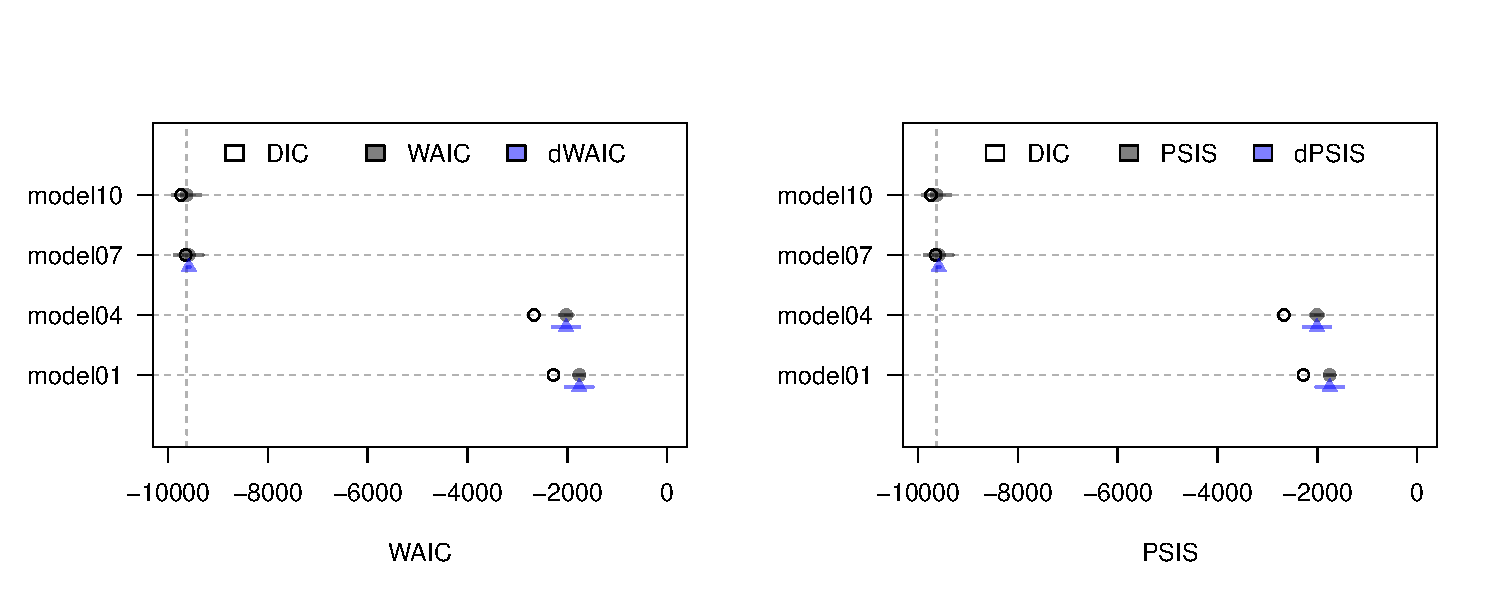
\includegraphics{index_files/figure-pdf/fig-rq1-waic-psis-1.pdf}

}

\caption{\label{fig-rq1-waic-psis}\textcolor{blue}{Comparison plot for selected models.
\textbf{\emph{Note:}} Open, black and blue points describe the posterior
means for the criteria. Continuous colored horizontal lines indicate the
criteria associated uncertainty.}}

\end{figure}%

Upon closer examination, the reasons behind the observed disparities in
the models become more apparent. \textcolor{blue}{Specifically,
Figure~\ref{fig-rq1-pred-speaker} demonstrates that the Normal LMM, as
outlined in Model \(4\), fails to adequately capture the data's
underlying patterns, resulting in predictions that are physically
inconsistent. This issue is illustrated by the \(95\%\) Highest
Probability Density Intervals (HPDI) extending beyond the expected zero
to one outcome range. Further insight into this lack of fit is provided
by Figure~\ref{fig-rq1-pred-speaker_model04}. The figure displays score
prediction densities for Model \(4\) that bear no resemblance to the
actual data densities.} Furthermore, the top two panels in
Figure~\ref{fig-rq1-model-outliers} reveal that misspecification in the
Normal LMM causes the model to be \emph{more surprised} by `extreme'
entropy scores, leading to their identification as highly unlikely and
influential observations. Consequently, the model is rendered unreliable
due to the potential biases present in the parameter estimates. In
contrast, the Beta-proportion GLLAMM appears to effectively capture the
data patterns, generating predictions within the expected data range.
This is evident in Figure~\ref{fig-rq1-pred-speaker} and complemented by
Figure~\ref{fig-rq1-pred-speaker_model10} and
Figure~\ref{fig-rq1-model-outliers}. In
Figure~\ref{fig-rq1-pred-speaker_model10}, Model \(10\) display
prediction densities that bear more resemblance to the actual data
densities. Furthermore, the bottom two panels in
Figure~\ref{fig-rq1-model-outliers} show the model is \emph{less
surprised} by `extreme' scores, fostering more trust in the model's
estimates.

\phantomsection\label{cell-fig-rq1-pred-speaker}
\begin{figure}[H]

\centering{

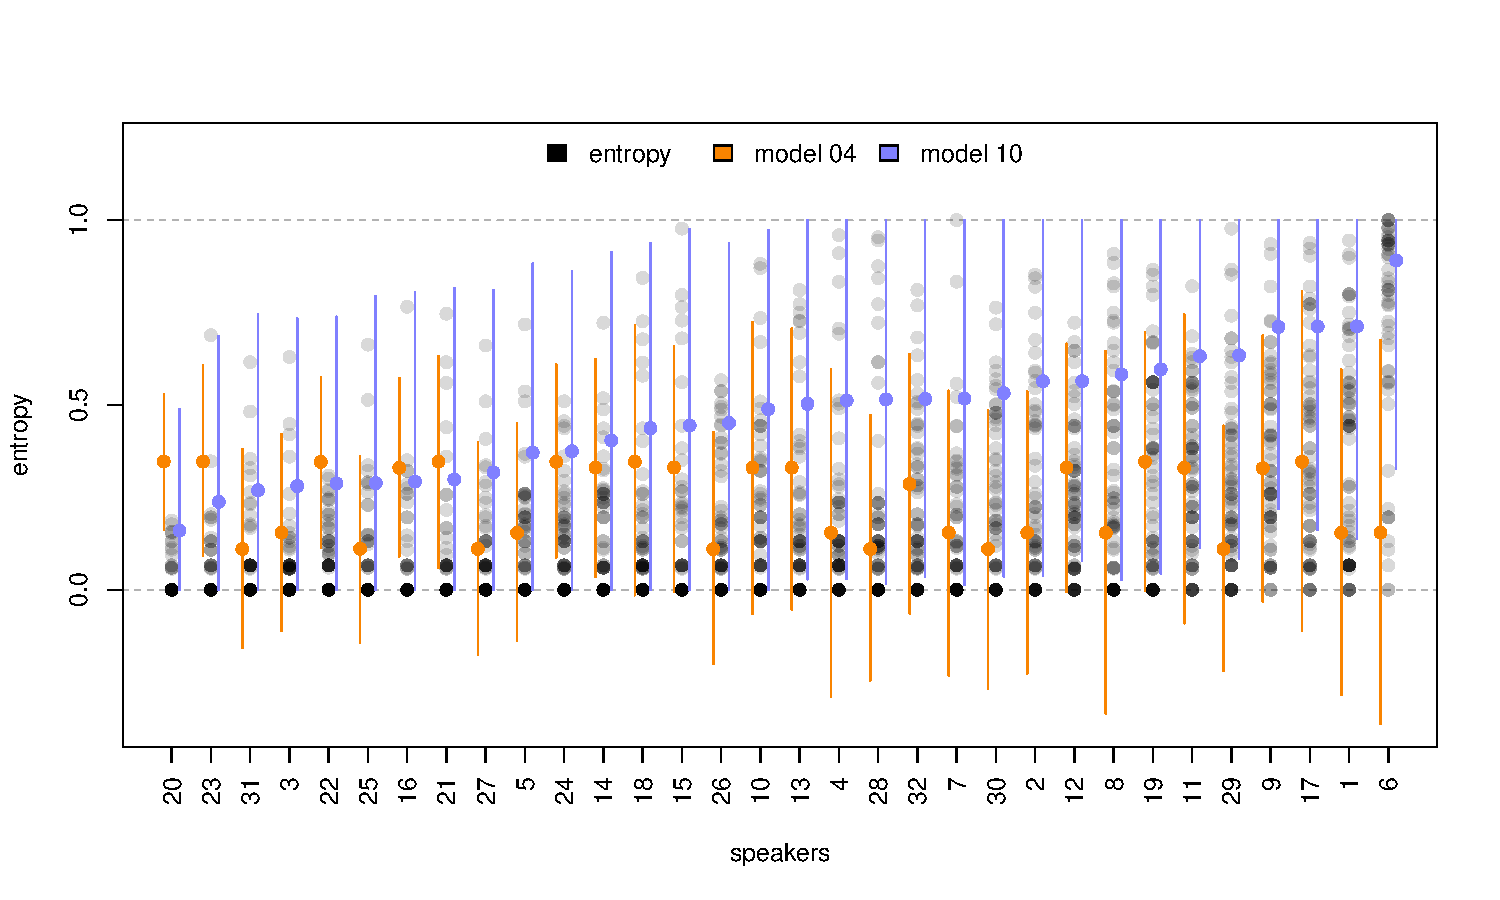
\includegraphics{index_files/figure-pdf/fig-rq1-pred-speaker-1.pdf}

}

\caption{\label{fig-rq1-pred-speaker}Entropy scores prediction for
selected models. \textcolor{blue}{\textbf{\emph{Note:}} Black points show manifest
entropy scores where darker points indicate greater overlap. Orange dots
and vertical lines show the posterior mean and 95\% HPDI derived from
Model 4. Blue dots and vertical lines show similar information from
Model 10.}}

\end{figure}%

\subsection{Estimation of speakers' latent potential intelligibility
from manifest entropy scores (RQ2)}\label{sec-R-RQ2}

The second research question aimed to demonstrate the application of the
Beta-proportion GLLAMM in estimating the latent potential
intelligibility of speakers. This was achieved by employing the general
mathematical formalism outlined in
Equation~\ref{eq-beta-GLLAMM-structural}, along with additional
specifications provided in Table~\ref{tbl-fitted}. The Bayesian
procedure successfully estimated the latent potential intelligibility of
speakers under Model \(10\) through the structural equation:

\begin{equation}\phantomsection\label{eq-beta-GLLAMM-structural-model10}{
SI_{i} = \alpha + e_{i} + u_{i}
}\end{equation}

Moreover, due to its implementation under Bayesian procedures, Model
\(10\) provides the complete posterior distribution of the speakers'
potential intelligibility scores. This provision, in turn, (1) enables
the calculation of summaries, facilitating the ranking of individuals,
and (2) supports the assessment of differences among selected speakers.
In both cases, the model considers the inherent uncertainty of the
estimates resulting from its measurement using multiple entropy scores.

\phantomsection\label{cell-fig-rq2-si-model10}
\begin{figure}[H]

\centering{

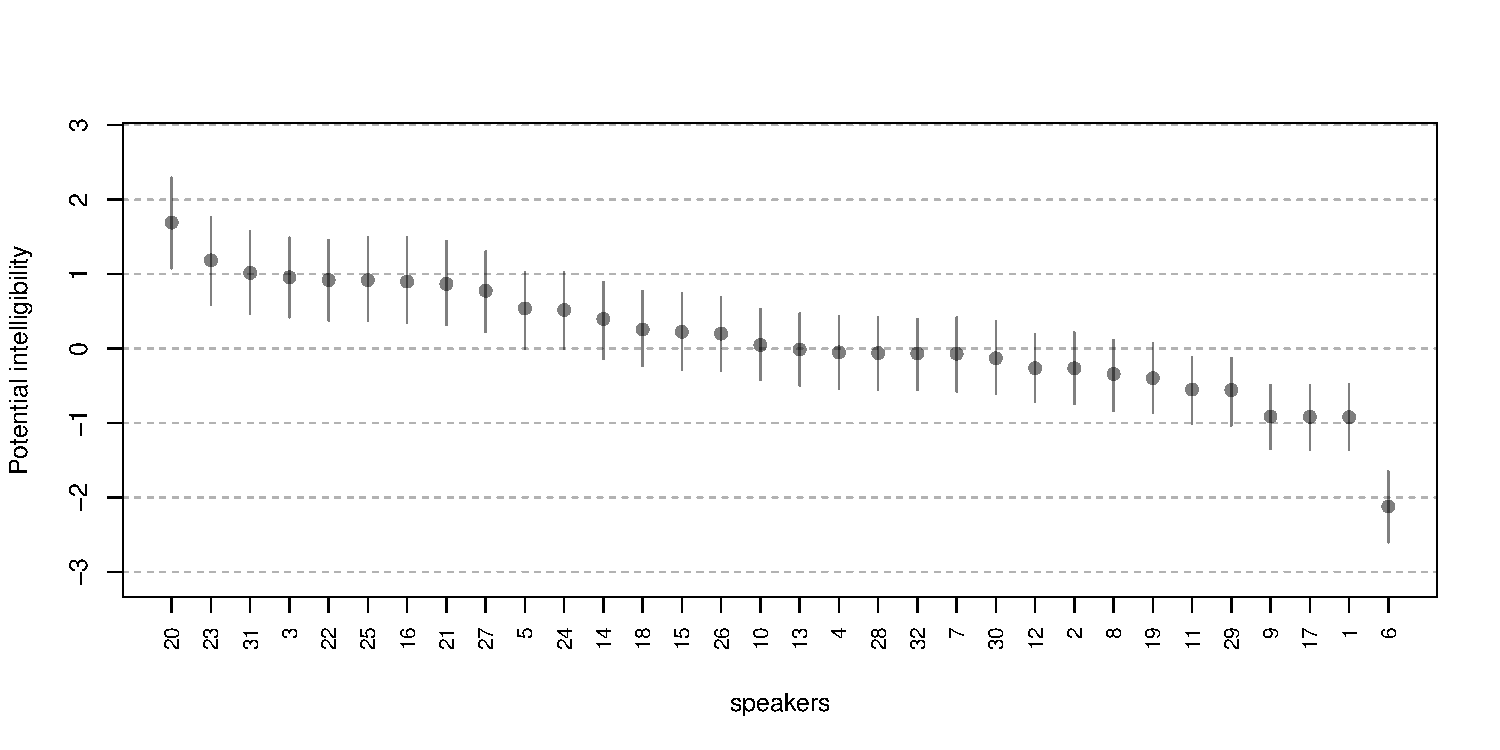
\includegraphics{index_files/figure-pdf/fig-rq2-si-model10-1.pdf}

}

\caption{\label{fig-rq2-si-model10}Model 10, latent potential
intelligibility of speakers. \textcolor{blue}{\textbf{\emph{Note:}} Black dots and
vertical lines show the posterior means and 95\% HPDI intervals.}}

\end{figure}%

\textcolor{blue}{Figure~\ref{fig-rq2-si-model10} displays the ranking of speakers in
decreasing order based on the posterior means of the latent potential
intelligibility. These estimates are accompanied by their associated
\(95\%\) HPDI.} The figure clearly indicate that speaker \(6\) stands
out as the least intelligible in the sample, followed farther behind by
speaker \(1\), \(17\) and \(9\). In contrast, the figure highlights
speaker \(20\) as the most intelligible, closely followed by speakers
\(23\), \(31\) and \(3\). \textcolor{blue}{Conversely, the full posterior distribution
for comparing potential intelligibility between the least and most
intelligible speakers against other selected speakers is shown in
Figure~\ref{fig-si_contr_model10}.} The figure reveals that only the
differences between speakers \(6\), \(1\), \(17\), and \(9\), along with
the difference between speakers \(20\) and \(3\) are statistically
significant, as their associated \(95\%\) HPDI did not overlap with zero
(shaded area). The R code to derive these scores and generate the figure
is available in the digital walk-through document (refer to
Section~\ref{sec-M-SM-OS} Open Science Statement).

\phantomsection\label{cell-fig-si_contr_model10}
\begin{figure}[H]

\centering{

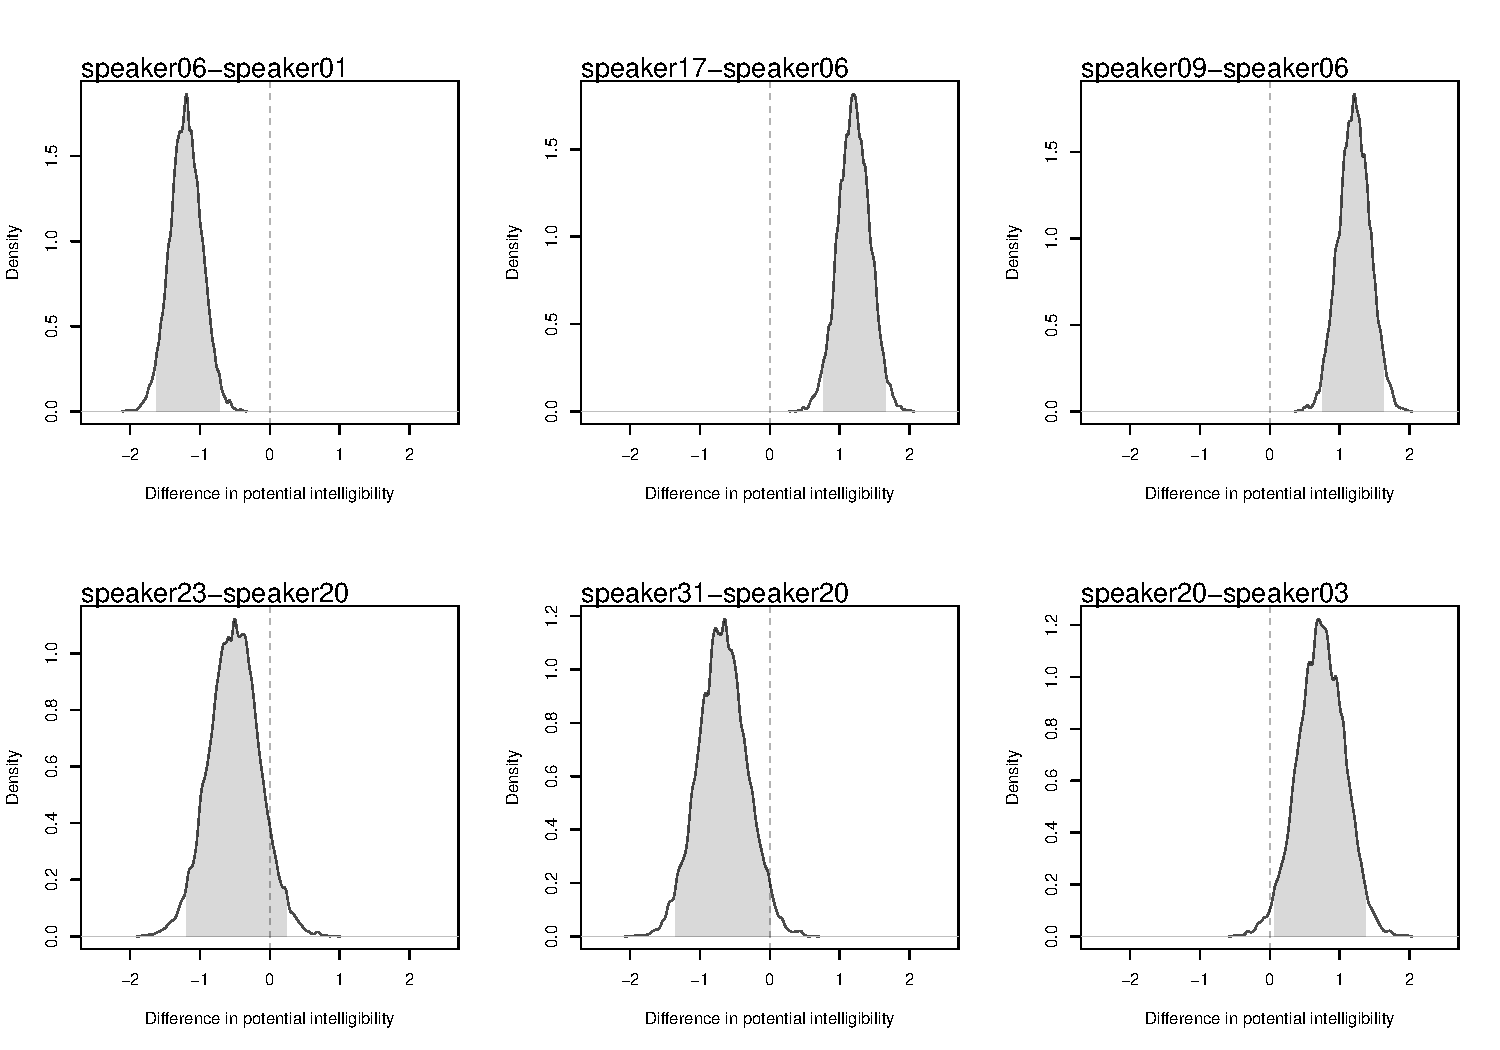
\includegraphics{index_files/figure-pdf/fig-si_contr_model10-1.pdf}

}

\caption{\label{fig-si_contr_model10}Model 10, potential intelligibility
comparisons among selected speakers. \textcolor{blue}{\textbf{\emph{Note:}} Shaded area
describes the 95\% HPDI.}}

\end{figure}%

\subsection{Testing the influence of speaker-related factors on
intelligibility (RQ3)}\label{sec-R-RQ3}

This research question illustrates how theories on intelligibility can
be examined within the model's framework. Specifically, the focus
centers on assessing the influence of speaker-related factors on
intelligibility, such as chronological age and hearing status. Notably,
despite RQ1 indicating the suitability of Beta-proportion GLLAMM models
for entropy scores, existing statistical literature suggests that, in
certain scenarios, models incorporating covariate adjustment exhibit
robustness to misspecification in the functional form linking an outcome
and covariates, commonly referred to as covariate-outcome relationship
\citep{Tackney_et_al_2023}. Consequently, this study compares all models
detailed in Table~\ref{tbl-fitted}. These models are characterized by
different covariate adjustments on entropy scores or the latent
potential intelligibility of speakers, namely chronological age and
hearing status, while potentially exhibiting misspecification in the
covariate-outcome relationship, as observed in the case of the Normal
LMM.

Similar to RQ1, all criteria consistently identify the Beta-proportion
GLLAMM outlined in models \(11\), \(12\) and \(10\) as the most
plausible models for the data. The models exhibit the lowest values for
both \texttt{WAIC} and \texttt{PSIS}, establishing them as the least
deviating models among those under comparison. Moreover,
Figure~\ref{fig-rq3-waic-psis} depicts with horizontal blue lines the
non-overlapping uncertainty for the models' \texttt{dWAIC} and
\texttt{dPSIS} values. This reveals that, when compared to Model \(11\),
most models exhibit significantly distinct predictive capabilities.
Models \(12\) and \(10\), however, stand out as exceptions to this
pattern. This observation suggests that Models \(11\), \(12\), and
\(10\) display the least deviation from \emph{perfect} predictive
accuracy in contrast to the other models. Lastly, the \texttt{weight} of
evidence in Tables Table~\ref{tbl-rq3-waic} and
Table~\ref{tbl-rq3-psis}, underscores that Model \(11\) accumulated the
greatest support, followed by Model \(12\), and lastly, by Model \(10\).

\phantomsection\label{cell-fig-rq3-waic-psis}
\begin{figure}[H]

\centering{

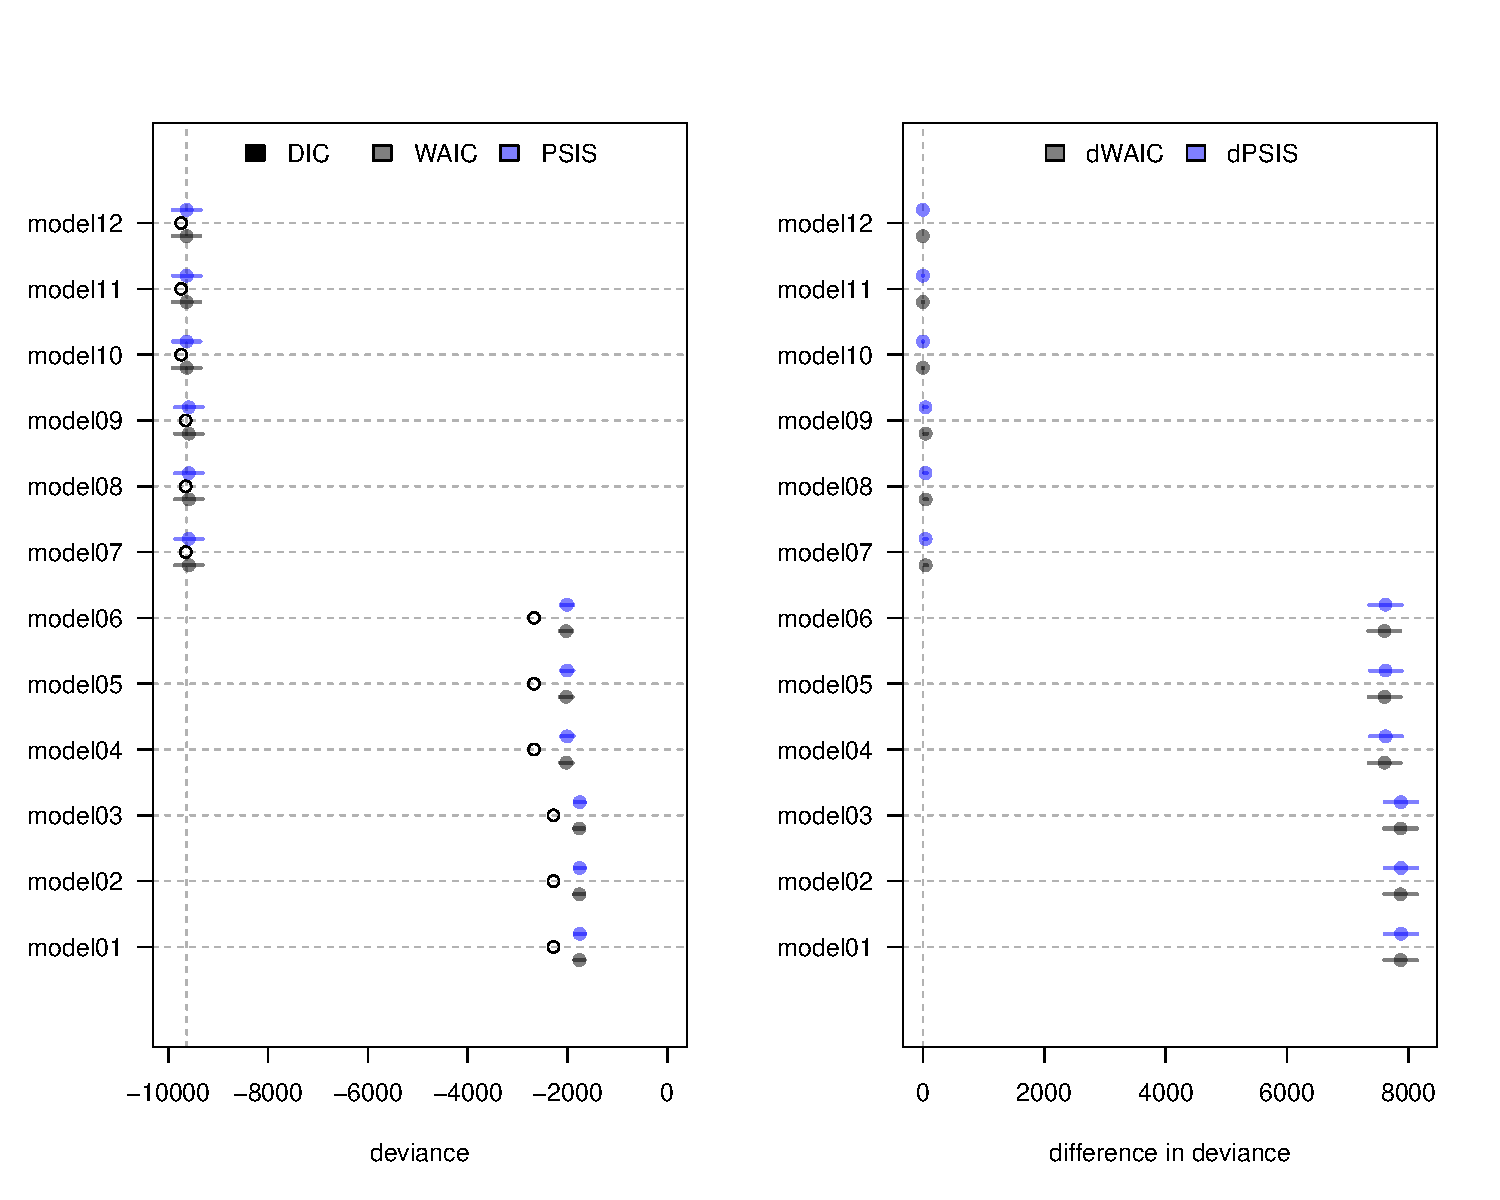
\includegraphics{index_files/figure-pdf/fig-rq3-waic-psis-1.pdf}

}

\caption{\label{fig-rq3-waic-psis}\textcolor{blue}{Comparison plot for all models.
\textbf{\emph{Note:}} Open, black and blue points describe the posterior
means for the criteria. Continuous colored horizontal lines indicate the
criteria associated uncertainty.}}

\end{figure}%

A closer examination of two models within this comparison set reveal the
reasons behind the largest observed disparities. The Normal LMM, as
outlined in Model \(6\), continues to face challenges in capturing
underlying data patterns, resulting in predictions that are physically
inconsistent, falling outside the outcome's range. Additionally, the
model persists in identifying highly unlikely and influential
observations, making it inherently unreliable. In contrast, the
Beta-proportion GLLAMM described by Model \(12\) appears to be less
susceptible to `extreme' scores, effectively capturing data patterns
within the expected data range and thereby instilling greater confidence
in the reliability of the model's estimates. This contrast is visually
depicted in Figure~\ref{fig-rq3-pred-speaker},
Figure~\ref{fig-rq3-pred-speaker_model06},
Figure~\ref{fig-rq3-pred-speaker_model12}, and
Figure~\ref{fig-rq3-model-outliers}.

Considering the results in Figure~\ref{fig-rq3-waic-psis}, the model
comparisons favor three distinct models: Model \(10\), \(11\) and
\(12\). Model \(10\), supported by \(20.4\%\) of the evidence, estimates
a single intercept \(\alpha\) and no slope to explain the potential
intelligibility of speakers (refer to
Table~\ref{tbl-parameter-model10}). In contrast, supported by \(45.1\%\)
of the evidence, Model \(11\) in Table~\ref{tbl-parameter-model11}
estimates distinct intercepts for each hearing status group, namely
\(\alpha_{HS[1]}\) for NH speakers and \(\alpha_{HS[2]}\) for the HI/CI
counterparts, while maintaining a single slope that gauges the impact of
age on potential intelligibility estimates. The \(95\%\) HPDI for the
comparison of intercepts \(\alpha_{HS[2]}-\alpha_{HS[1]}\) reveal
significant differences between NH and HI/CI speakers. Lastly, with
evidence of \(34.1\%\), Model \(12\) in
Table~\ref{tbl-parameter-model12} estimates one intercept and slope per
hearing status group, namely \(\alpha_{HS[1]}\) and \(\beta_{A,HS[1]}\)
for the NH speakers, and \(\alpha_{HS[2]}\) and \(\beta_{A,HS[2]}\) for
the HI/CI counterparts. The \(95\%\) HPDI for the comparison of
intercepts and slopes reveal significant differences solely in the
slopes between NH and their HI/CI counterparts
(\(\beta_{A,HS[2]}-\beta_{A,HS[1]}\)).

However, a discerning reader can notice that these models yield
conflicting conclusions regarding the influence of chronological age and
hearing status on intelligibility. Model \(10\) implies no influence of
chronological age and hearing status on the potential intelligibility of
speakers. A visual inspection of
Figure~\ref{fig-rq3-intelligibility-model10}, however, reveals the
reason for the model's low support. Model \(10\) fails to capture the
prevalent increasing age pattern observed in potential intelligibility
estimates. In contrast, Model \(11\) identifies significant differences
in potential intelligibility between NH and HI/CI speakers. The model
further suggests that with the progression of chronological age, HI/CI
speakers lag behind in intelligibility development, with no opportunity
to catch up to their NH counterparts within the analyzed age range, as
depicted in Figure~\ref{fig-rq3-intelligibility-model11}. Finally, Model
\(12\) indicates no significant differences in intelligibility between
NH and HI/CI speakers at \(68\) months of age (around \(6\) years old).
However, the model reveals distinct evolution patterns of
intelligibility per unit of chronological age between different hearing
status groups, with HI/CI speakers displaying a slower rate of
development compared to their NH counterparts within the analyzed age
range. The latter is evident in
Figure~\ref{fig-rq3-intelligibility-model12}.

\begin{longtable}[]{@{}ccc@{}}

\caption{\label{tbl-parameter-model10}\textcolor{blue}{Model 10, parameter estimates and
95\% HPDI.}}

\tabularnewline

\toprule\noalign{}
Parameter & Posterior mean & 95\% HPDI \\
\midrule\noalign{}
\endhead
\bottomrule\noalign{}
\endlastfoot
\(\alpha\) & 0.01 & {[}-0.09, 0.1{]} \\

\end{longtable}

\phantomsection\label{cell-fig-rq3-intelligibility-model10}
\begin{figure}[H]

\centering{

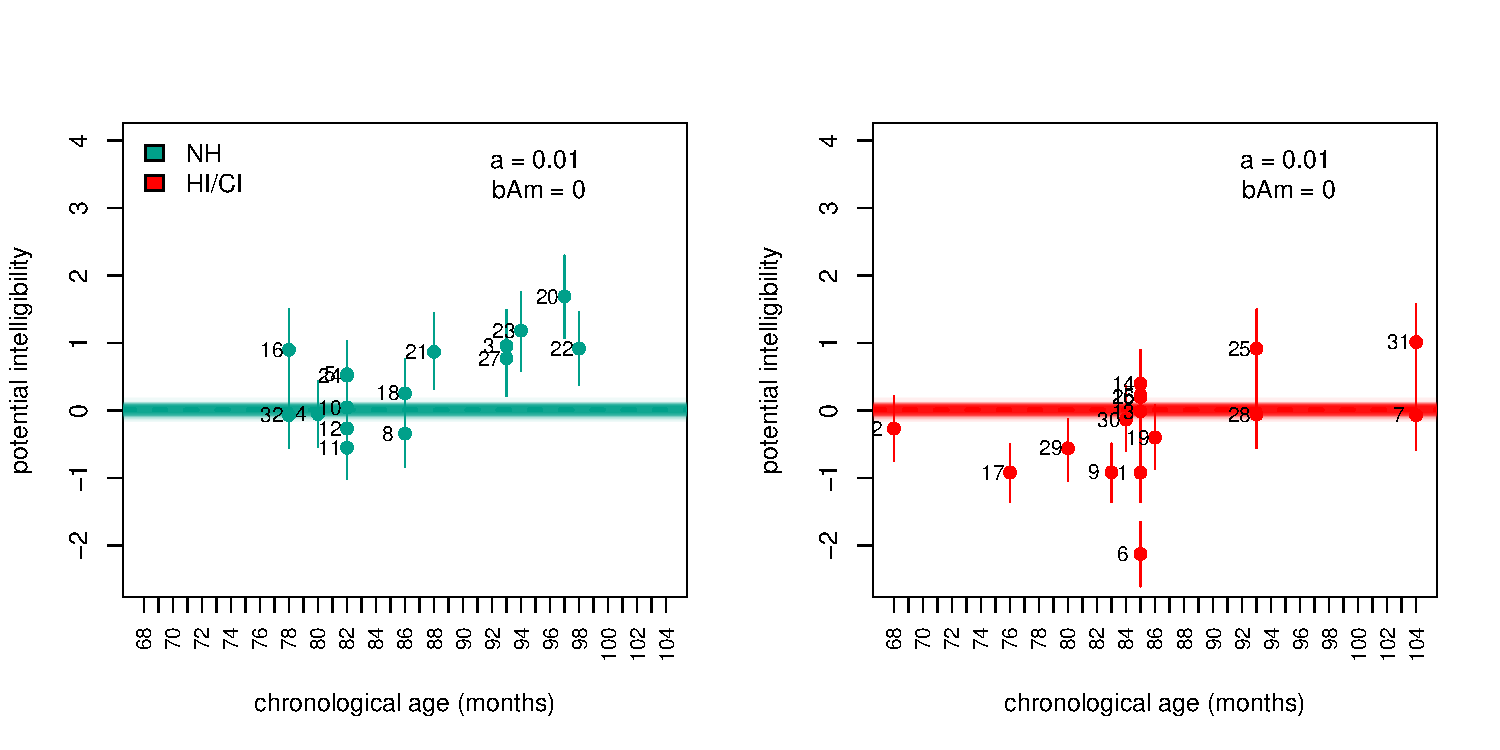
\includegraphics{index_files/figure-pdf/fig-rq3-intelligibility-model10-1.pdf}

}

\caption{\label{fig-rq3-intelligibility-model10}Model 10, Potential
intelligibility per chronological age and hearing status.
\textcolor{blue}{\textbf{\emph{Note:}} Colored dots denote the posterior means, vertical
lines describe the 95\% HPDI, thick discontinuous line indicate the
regression line, thin continuous lines denote regression lines samples
from the posterior distribution, and numbers indicate the speaker
index.}}

\end{figure}%

\begin{longtable}[]{@{}ccc@{}}

\caption{\label{tbl-parameter-model11}\textcolor{blue}{Model 11, parameter estimates and
95\% HPDI.}}

\tabularnewline

\toprule\noalign{}
Parameter & Posterior mean & 95\% HPDI \\
\midrule\noalign{}
\endhead
\bottomrule\noalign{}
\endlastfoot
\(\alpha\) & 0.01 & {[}-0.08, 0.11{]} \\
\(\alpha_{HS[1]}\) & 0.53 & {[}0.11, 0.94{]} \\
\(\alpha_{HS[2]}\) & -0.03 & {[}-0.43, 0.39{]} \\
\(\beta_{A}\) & 0.07 & {[}0.05, 0.1{]} \\
& & \\
Contrasts & & \\
\(\alpha_{HS[2]} - \alpha_{HS[1]}\) & -0.55 & {[}-1, -0.15{]} \\

\end{longtable}

\phantomsection\label{cell-fig-rq3-intelligibility-model11}
\begin{figure}[H]

\centering{

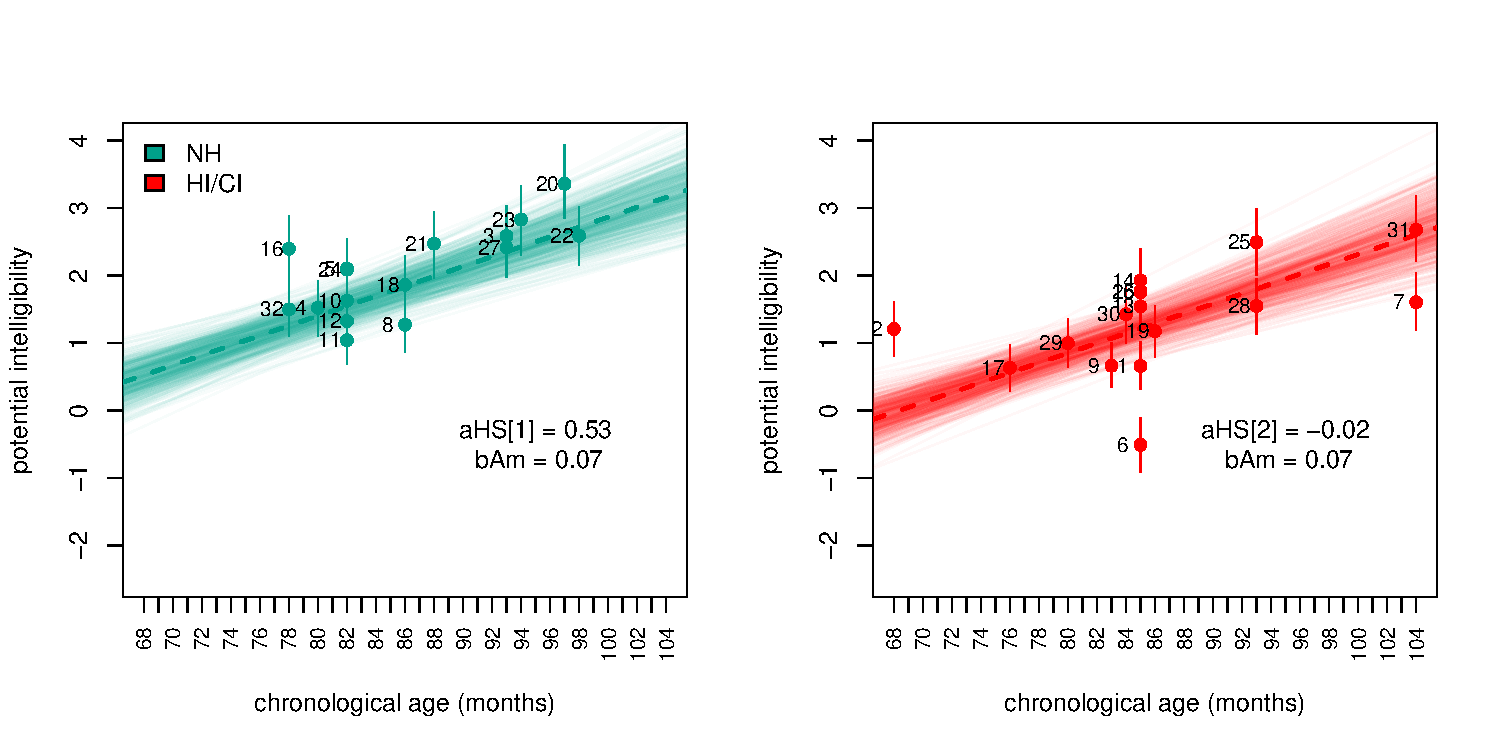
\includegraphics{index_files/figure-pdf/fig-rq3-intelligibility-model11-1.pdf}

}

\caption{\label{fig-rq3-intelligibility-model11}Model 11, Potential
intelligibility per chronological age and hearing status.
\textcolor{blue}{\textbf{\emph{Note:}} Colored dots denote the posterior means, vertical
lines describe the 95\% HPDI, thick discontinuous line indicate the
regression line, thin continuous lines denote regression lines samples
from the posterior distribution, and numbers indicate the speaker
index.}}

\end{figure}%

\begin{longtable}[]{@{}ccc@{}}

\caption{\label{tbl-parameter-model12}\textcolor{blue}{Model 12, parameter estimates and
95\% HPDI.}}

\tabularnewline

\toprule\noalign{}
Parameter & Posterior mean & 95\% HPDI \\
\midrule\noalign{}
\endhead
\bottomrule\noalign{}
\endlastfoot
\(\alpha\) & 0.01 & {[}-0.09, 0.11{]} \\
\(\alpha_{HS[1]}\) & 0.21 & {[}-0.28, 0.72{]} \\
\(\alpha_{HS[2]}\) & 0.23 & {[}-0.24, 0.69{]} \\
\(\beta_{A,HS[1]}\) & 0.10 & {[}0.07, 0.13{]} \\
\(\beta_{A,HS[2]}\) & 0.06 & {[}0.03, 0.09{]} \\
& & \\
Contrasts & & \\
\(\alpha_{HS[2]} - \alpha_{HS[1]}\) & 0.01 & {[}-0.61, 0.74{]} \\
\(\beta_{A,HS[2]} - \beta_{A,HS[1]}\) & -0.04 & {[}-0.08, 0{]} \\

\end{longtable}

\phantomsection\label{cell-fig-rq3-intelligibility-model12}
\begin{figure}[H]

\centering{

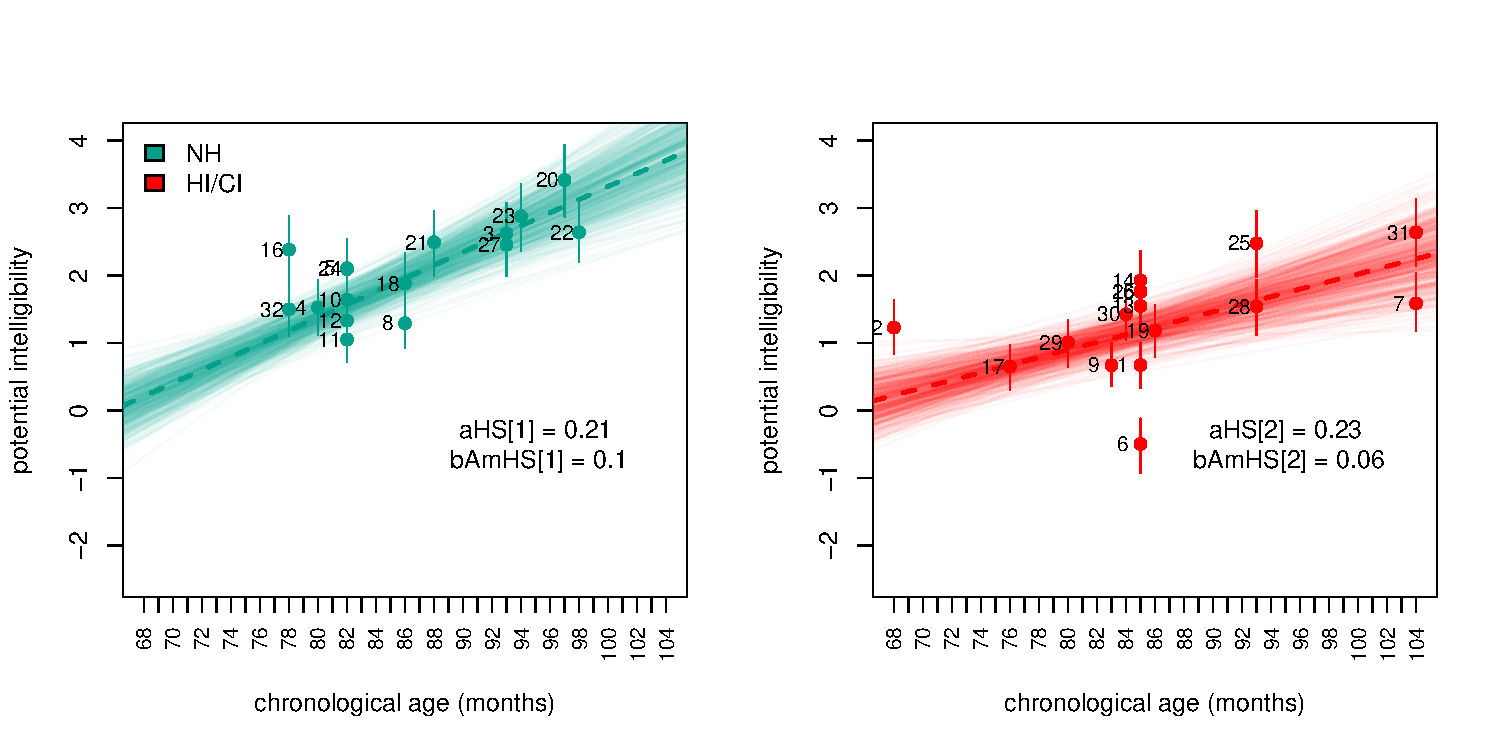
\includegraphics{index_files/figure-pdf/fig-rq3-intelligibility-model12-1.pdf}

}

\caption{\label{fig-rq3-intelligibility-model12}Model 12, Potential
intelligibility per chronological age and hearing status.
\textcolor{blue}{\textbf{\emph{Note:}} Colored dots denote the posterior means, vertical
lines describe the 95\% HPDI, thick discontinuous line indicate the
regression line, thin continuous lines denote regression lines samples
from the posterior distribution, and numbers indicate the speaker
index.}}

\end{figure}%

\section{Discussion}\label{sec-discussion}

\subsection{Findings}\label{sec-D-F}

This study examined the suitability of the Bayesian Beta-proportion
GLLAMM for the quantitative measuring and testing of research theories
related to speech intelligibility using entropy scores. The initial
findings supported the assertion that Beta-proportion GLLAMMs
consistently outperformed Normal LMMs in predicting entropy scores,
underscoring its superior predictive performance. The results emphasized
that models neglecting the outcomes' measurement error and boundedness
lead to underfitting and misspecification issues, even when robust
features are integrated. This is clearly illustrated by the Normal LMMs.

Secondly, the study showcased the Beta-proportion GLLAMM's proficiency
in estimating the latent potential intelligibility of speakers based on
manifest entropy scores. Implemented under Bayesian procedures, the
proposed model offered a valuable advantage over frequentist methods by
further providing the full posterior distribution of the speakers'
potential intelligibility. This provision facilitated the calculation of
summaries, aiding individual rankings, and supported the comparisons
among selected speakers. In both scenarios, the proposed model accounted
for the inherent uncertainty in the intelligibility estimates.

Thirdly, the study illustrated how the proposed model assessed the
impact of speaker-related factors on potential intelligibility. The
results suggested that multiple models were plausible for the observed
entropy scores, indicating that different speaker-related factor
theories were viable for the data, with some presenting contradictory
conclusions about the influence of those factors on intelligibility.
However, even when unequivocal support for one theory was not possible,
the divided support among these models informed that certain statistical
issues may be hindering the model's ability to distinguish among
individuals and, ultimately, among models. These issues encompassed the
insufficient sample size of speakers, the inadequate representation of
the population of speakers, and the imprecise measurement of the latent
variable of interest.

Ultimately, this study introduced researchers to innovative statistical
tools that enhanced existing research models. These tools not only
assessed the predictability of empirical phenomena but also
quantitatively measured the latent trait of interest, namely potential
intelligibility, facilitating the comparison of research theories
related to this trait. However, the presented tools introduce new
challenges for researchers seeking their implementation. These
challenges emerge from two distinct aspects: one methodological and the
other practical. In the methodological domain, researchers need
familiarity with Bayesian methods and the principled formulation of
assumptions regarding the data-generating process and research
inquiries. This entails understanding and addressing each of the data
and research challenges within the context of a statistical
(probabilistic) model. Conversely, in the practical domain, researchers
need familiarity with probabilistic programming languages (PPLs), which
are designed for specifying and obtaining inferences from probabilistic
models -the core of Bayesian methods. To ensure the successful
utilization of this new statistical tool, this study addresses both
challenges by providing comprehensive, step-by-step guidance in the form
of a digital walk-through document (refer to Section~\ref{sec-M-SM-OS}
Open Science Statement).

\subsection{Limitations and further research}\label{sec-D-LFR}

This study provides valuable insights into the use of a novel approach
to simultaneously address the different data features of entropy scores
in speech intelligibility research. However, it is important to
acknowledge the limitations of this study and explore potential avenues
for future research. Firstly, the study interprets potential
intelligibility as an unobserved latent trait of speakers influencing
the likelihood of observing a set of entropy scores. These scores, in
turn, reflect the transcribers' ability to decode words in sentences
produced by the same speakers. Despite this practical approach, the
construct validity of the latent trait heavily depends on the listeners'
appropriate understanding and execution of the transcription task.
Construct validity, as defined by \citet{Cronbach_et_al_1955}, refers to
the extent to which a set of manifest variables accurately represents a
concept that cannot be directly measured. Considering the study assumes
the transcription task set by \citet{Boonen_et_al_2021} was properly
understood and executed, it expects that potential intelligibility
reflects the overall speech intelligibility of speakers. However, the
study does not delve into the general epistemological considerations
regarding the connection between the latent variable and the concept.

Secondly, the study revealed a notable lack of unequivocal support for
one of the models among the compared set. This outcome may be attributed
to factors such as the insufficient sample size of speakers, the
inadequate representation of the populations of speakers (referred to as
selection bias), and the imprecise measurement of the latent variable.
Small sample size and selection bias yield data with limited outcome and
covariates ranges, leading to biased and imprecise parameter estimates
\citep{Everitt_et_al_2010}. Moreover, fueled by the reduced measurement
precision, these issues can result in models with diminished statistical
power and a higher risk of type I or type II errors
\citep{McElreath_2020}. \textcolor{blue}{Consequently, future research should consider
extending this study by conducting formal sample size planning. This
entails assessing the impact of expanding the speakers' pool on testing
research theories or increasing the number of speech samples,
transcriptions, and listeners to enhance the precision of the potential
intelligibility estimates. With these insights, future investigations
could contemplate increasing the speaker sample with a group that
adequately represents the population of interest.} However, this must be
done while mindful of the pragmatic limitations associated with
transcription tasks, specifically considering the costs and
time-intensiveness of the procedure.

Thirdly, the study presented an illustrative example for the
investigation of research theories within the model's framework.
However, it did not offer an exhaustive evaluation of all factors
influencing intelligibility, which are thoroughly explored in the works
of \citet{Niparko_et_al_2010}, \citet{Boons_et_al_2012},
\citet{Gillis_2018}, and \citet{Fagan_et_al_2020}. Consequently, the
study cannot discard the presence of unobservable variables that might
bias the parameter estimates, potentially impacting the inferences
provided. Hence, future research should consider integrating appropriate
causal hypotheses about these factors into the proposed models, as
proper covariate adjustment facilitates the production of unbiased and
precise parameter estimates
\citep{Cinelli_et_al_2021, Deffner_et_al_2022}.

Lastly, this study proposes two directions for future exploration in
speech intelligibility research. Firstly, there is an opportunity to
investigate alternative methods for assessing speech intelligibility
beyond transcription tasks and entropy scores. The experimental design
of transcription tasks imply that the procedure may be time-intensive
and costly. Thus, exploring less time-intensive or more cost-effective
procedures, that still offer comparable precision in intelligibility
estimates, could benefit both researchers and speech therapists alike.
An illustrative example of such a method is Comparative Judgment (CJ),
where judges compare and score the perceived intensity of a trait
between two stimuli \citep{Thurstone_1927}. In the context of the
intelligibility trait, the stimuli under assessment could be the speech
samples uttered by two speakers. Nevertheless, CJ serve as an ideal
example as the method has gained increasing attention within the realm
of educational assessment, with several studies providing evidence for
its validity in assessing various task within student works, as
demonstrated by examples in \citet{Pollitt_2012a};
\citet{Pollitt_2012b}, \citet{Lesterhuis_2018}, \citet{vanDaal_2020},
and \citet{Verhavert_et_al_2019}.

Conversely, a second avenue for exploration involves integrating diverse
data types and evaluation methods to assess individuals'
intelligibility. This can be accomplished by leveraging two features of
Bayesian methods: their flexibility and the concept of Bayesian
updating. Bayesian methods possess the flexibility to simultaneously
handle various data types. Additionally, through Bayesian updating,
researchers can integrate information from the posterior distribution of
parameters as priors in models for subsequent evaluations. Ultimately,
this could enable researchers to assess speakers' intelligibility
progress without committing to a specific data type or evaluation
method. This advancement could mirror the emergence of second-generation
Structural Equation Models proposed by \citet{Muthen_2001}, where models
facilitate the combined estimation of categorical and continuous latent
variables. However, in the context of future research, the proposal
would facilitate the estimation of latent variables using a combination
of data types and evaluation methods, contingent upon the fulfillment of
construct validity by those evaluation methods.

\section{Conclusion}\label{sec-conclusion}

This study highlights the effectiveness of the Bayesian Beta-proportion
GLLAMM to collectively address several key data features when
investigating unobservable and complex traits, using speech
intelligibility and entropy scores as an example. The results
demonstrate the proposed model consistently outperforms the Normal LMM
in predicting the empirical phenomena. Moreover, it exhibits the ability
to quantify the latent potential intelligibility of speakers, allowing
for the ranking and comparison of individuals based on the latent trait
while accommodating associated uncertainties. Additionally, the proposed
model facilitates the exploration of research theories concerning the
influence of speaker-related factors on potential intelligibility. The
study indicates that integrating and comparing these theories within the
model's framework is a straightforward task.

However, the introduction of these innovative statistical tools presents
new challenges for researchers seeking implementation. These challenges
encompass the principled formulation of assumptions about the
data-generating processes and research inquiries, along with the need
for familiarity with probabilistic programming languages (PPLs)
essential for implementing Bayesian methods. Nevertheless, the study
suggests several promising avenues for future research, including power
analysis, causal hypothesis formulation, and exploration and integration
of novel evaluation methods for assessing intelligibility. The insights
derived from this study hold implications for both researchers and data
analysts interested in quantitatively measuring and testing theories
related to nuanced, unobservable constructs, while also considering the
appropriate prediction of the empirical phenomena.

\newpage{}

\section*{Declarations}\label{declarations}
\addcontentsline{toc}{section}{Declarations}

\textbf{Funding:} The project was founded through the Research Fund of
the University of Antwerp (BOF).

\textbf{Conflict of interests:} The authors declare no conflict of
interest.

\textbf{Ethics approval:} This is an observational study. The University
of Antwerp Research Ethics Committee has confirmed that no ethical
approval is required.

\textbf{Consent to participate:} Not applicable

\textbf{Consent for publication:} All authors have read and agreed to
the published version of the manuscript.

\textbf{Availability of data and materials:} \textcolor{blue}{The data is delivered upon
request.}

\textbf{Code availability:} \textcolor{blue}{All the code utilized in this research is
available in the different notebooks and \texttt{CODE\ LINKS} referenced
in the digital document. The digital document is located at:}
\url{https://jriveraespejo.github.io/paper1_manuscript/}.

\textbf{Authors' contributions:} \emph{Conceptualization:} S.G., S.dM.,
and J.M.R.E; \emph{Data curation:} J.M.R.E.; \emph{Formal Analysis:}
J.M.R.E.; \emph{Funding acquisition:} S.G. and S.dM;
\emph{Investigation:} S.G.; \emph{Methodology:} S.G., S.dM., and
J.M.R.E; \emph{Project administration:} S.G. and S.dM.;
\emph{Resources:} S.G. and S.dM.; \emph{Software: J.M.R.E.};
\emph{Supervision:} S.G. and S.dM.; \emph{Validation:} J.M.R.E.;
\emph{Visualization:} J.M.R.E.; \emph{Writing - original draft:}
J.M.R.E.; \emph{Writing - review \& editing:} S.G. and S.dM.

\newpage{}

\section{Appendix}\label{sec-appendix}

\subsection{Entropy scores calculation}\label{sec-appA}

This section exemplifies the entropy calculation procedure. \textcolor{blue}{For that
purpose, the words in position two, three, four and five observed in
Table~\ref{tbl-alignment} were used. These words were assumed present in
the first sentence, produced by the first speaker assigned to the first
block, and transcribed by five listeners (\(w=\{2,3,4,5\}\), \(s=1\),
\(i=1\), \(b=1\), \(J=5\)). For second word, the first four listeners
identified the word type \emph{jongen} \((T_{j1})\), while the last
identified the word type \emph{hond} \((T_{j2})\).} Therefore, two word
types were identified (\(K=2\)), with proportions equal to
\(\{ p_{1}, p_{2} \}\) \(=\) \(\{ 4/5, 1/5 \}\) \(=\)
\(\{ 0.8, 0.2 \}\), and entropy score equal to:

\[ 
H_{2111} = \frac{ -\left[ 0.8 \cdot log_{2}(0.8) + 0.2 \cdot log_{2}(0.2) \right] }{ log_{2}(5)} \approx 0.3109
\]

\textcolor{blue}{For the fourth word, two listeners identified the word type \emph{een}
\((T_{j1})\), one listener the word type \emph{de} \((T_{j2})\), and
another the word \emph{geen} \((T_{j3})\).} A blank space \emph{{[}B{]}}
is a symbol that defines the absence of a word in a space where a word
is expected, as compared with other transcriptions, during the alignment
procedure. Notice that for calculation purposes, because the blank space
is not expected in such position, this is considered as a different word
type. Consequently four word types were registered (\(K=4\)), with
proportions equal to \(\{ p_{1}, p_{2}, p_{3}, p_{4} \}\) \(=\)
\(\{ 2/5, 1/5, 1/5, 1/5 \}\) \(=\) \(\{ 0.4, 0.2, 0.2, 0.2 \}\) and
entropy score equal to:

\[ 
H_{4111} = \frac{ -\left[ 0.4 \cdot log_{2}(0.4) + 3 \cdot 0.2 \cdot log_{2}(0.2) \right] }{ log_{2}(5)} \approx 0.8277
\] \textcolor{blue}{For the fifth word, each listener transcribed a different word.} It
is important to highlight that when a listener does not identify a
complete word, or part of it, (s)he is instructed to write
\emph{{[}X{]}} in that position. However, for the calculation of the
entropy score, if more than one listener marks an unidentifiable word
with \emph{{[}X{]}}, each one of them is considered a different word
type. This is done to avoid the artificial reduction of the entropy
score, as \emph{{[}X{]}} values already indicate the word's lack of
intelligibility. . Consequently, five word types were observed,
\(T_{j1}=\)\emph{kikker}, \(T_{j2}=\)\emph{{[}X{]}},
\(T_{j3}=\)\emph{kokkin}, \(T_{j4}=\)\emph{kikkers},
\(T_{j5}=\)\emph{{[}X{]}} (\(K=5\)), with proportions equal to
\(\{ p_{1}, p_{2}, p_{3}, p_{4}, p_{5} \}\) \(=\)
\(\{ 1/5, 1/5, 1/5, 1/5, 1/5 \}\) \(=\)
\(\{ 0.2, 0.2, 0.2, 0.2, 0.2 \}\), and entropy score equal to:

\[ 
H_{5111} = \frac{ -\left[ 5 \cdot 0.2 \cdot log_{2}(0.2) \right] }{ log_{2}(5)} = 1
\]

\textcolor{blue}{Lastly, for the third word, the first two listeners identified the word
type \emph{ziet} \((T_{j1})\), the next two listeners identified the
word type \emph{zag} \((T_{j2})\), while the last one identified the
word type \emph{zoekt} \((T_{j3})\). Consequently, three word types were
identified (\(K=3\)), with proportions equal to
\(\{ p_{1}, p_{2}, p_{3} \}\) \(=\) \(\{ 2/5, 2/5, 1/5 \}\) \(=\)
\(\{ 0.4, 0.4, 0.2 \}\), and entropy score equal to:}

\[
H_{2111} = \frac{ -\left[ 2 \cdot 0.4 \cdot log_{2}(0.4) + 0.2 \cdot log_{2}(0.2) \right] }{ log_{2}(5)} \approx 0.6555
\]

\textcolor{blue}{Importantly, this last example showcases the major difference between
entropy and measures of accuracy based on the percentage of
(un)intelligible words: entropy scores employ all word type proportions
in their calculations, effectively capturing the agreement and
disagreement among listeners' word transcriptions
\citep{Boonen_et_al_2021}. In contrast, the percentage of
(un)intelligible words mostly discards some word type proportions in
favor of \emph{simpler} agreement or disagreement percentages. For
example, an agreement percentage could be reflected by the proportion of
the most frequent word, i.e., \(\text{max}\{ 0.4, 0.4, 0.2 \}=0.4\), or
by other similar percentages detailed in the works of
\citet{Flipsen_2006} and \citet{Lagerberg_et_al_2014}.}

\newpage{}

\subsection{Tables}\label{sec-appB}

\begin{longtable}[]{@{}crrrrrrr@{}}

\caption{\label{tbl-rq1-waic}WAIC comparison for selected models.
\textcolor{blue}{\textbf{\emph{Note:}} The table is sorted based on \texttt{weight} from
most to least plausible model(s) for the data.}}

\tabularnewline

\toprule\noalign{}
Model & DIC & WAIC & SE & dWAIC & dSE & pWAIC & weight \\
\midrule\noalign{}
\endhead
\bottomrule\noalign{}
\endlastfoot
10 & -9741.66 & -9630.63 & 276.64 & 0.00 & NA & 55.52 & 1 \\
7 & -9649.54 & -9586.00 & 274.50 & 44.63 & 17.89 & 31.77 & 0 \\
4 & -2670.62 & -2024.84 & 127.02 & 7605.78 & 263.22 & 322.89 & 0 \\
1 & -2278.68 & -1761.10 & 101.80 & 7869.53 & 266.54 & 258.79 & 0 \\

\end{longtable}

\begin{longtable}[]{@{}crrrrrrr@{}}

\caption{\label{tbl-rq1-psis}PSIS comparison for selected models.
\textcolor{blue}{\textbf{\emph{Note:}} The table is sorted based on \texttt{weight} from
most to least plausible model(s) for the data.}}

\tabularnewline

\toprule\noalign{}
Model & DIC & PSIS & SE & dPSIS & dSE & pPSIS & weight \\
\midrule\noalign{}
\endhead
\bottomrule\noalign{}
\endlastfoot
10 & -9741.66 & -9629.27 & 276.74 & 0.00 & NA & 56.19 & 1 \\
7 & -9649.54 & -9585.92 & 274.56 & 43.36 & 17.67 & 31.81 & 0 \\
4 & -2670.62 & -2007.66 & 128.57 & 7621.61 & 263.60 & 331.48 & 0 \\
1 & -2278.68 & -1753.71 & 102.09 & 7875.57 & 266.54 & 262.48 & 0 \\

\end{longtable}

\begin{longtable}[]{@{}crrrrrrr@{}}

\caption{\label{tbl-rq3-waic}WAIC comparison for all models.
\textcolor{blue}{\textbf{\emph{Note:}} The table is sorted based on \texttt{weight} from
most to least plausible model(s) for the data.}}

\tabularnewline

\toprule\noalign{}
Model & DIC & WAIC & SE & dWAIC & dSE & pWAIC & weight \\
\midrule\noalign{}
\endhead
\bottomrule\noalign{}
\endlastfoot
11 & -9741.51 & -9632.24 & 276.80 & 0.00 & NA & 54.63 & 0.46 \\
12 & -9741.49 & -9631.66 & 276.82 & 0.58 & 1.00 & 54.91 & 0.34 \\
10 & -9741.66 & -9630.63 & 276.64 & 1.61 & 2.97 & 55.52 & 0.20 \\
9 & -9649.15 & -9586.67 & 274.35 & 45.56 & 18.01 & 31.24 & 0.00 \\
8 & -9649.05 & -9586.41 & 274.33 & 45.83 & 18.01 & 31.32 & 0.00 \\
7 & -9649.54 & -9586.00 & 274.50 & 46.24 & 18.19 & 31.77 & 0.00 \\
6 & -2669.28 & -2027.11 & 126.86 & 7605.13 & 263.15 & 321.08 & 0.00 \\
4 & -2670.62 & -2024.84 & 127.02 & 7607.40 & 263.22 & 322.89 & 0.00 \\
5 & -2669.28 & -2024.58 & 127.06 & 7607.66 & 263.24 & 322.35 & 0.00 \\
3 & -2279.58 & -1762.08 & 101.79 & 7870.16 & 266.68 & 258.75 & 0.00 \\
1 & -2278.68 & -1761.10 & 101.80 & 7871.14 & 266.64 & 258.79 & 0.00 \\
2 & -2279.35 & -1760.36 & 101.86 & 7871.88 & 266.69 & 259.49 & 0.00 \\

\end{longtable}

\begin{longtable}[]{@{}crrrrrrr@{}}

\caption{\label{tbl-rq3-psis}PSIS comparison for all models.
\textcolor{blue}{\textbf{\emph{Note:}} The table is sorted based on \texttt{weight} from
most to least plausible model(s) for the data.}}

\tabularnewline

\toprule\noalign{}
Model & DIC & PSIS & SE & dPSIS & dSE & pPSIS & weight \\
\midrule\noalign{}
\endhead
\bottomrule\noalign{}
\endlastfoot
11 & -9741.51 & -9631.16 & 276.88 & 0.00 & NA & 55.17 & 0.46 \\
12 & -9741.49 & -9630.70 & 276.90 & 0.47 & 1.01 & 55.39 & 0.36 \\
10 & -9741.66 & -9629.27 & 276.74 & 1.89 & 2.84 & 56.19 & 0.18 \\
9 & -9649.15 & -9586.58 & 274.41 & 44.58 & 17.91 & 31.28 & 0.00 \\
8 & -9649.05 & -9586.33 & 274.39 & 44.83 & 17.91 & 31.36 & 0.00 \\
7 & -9649.54 & -9585.92 & 274.56 & 45.24 & 18.10 & 31.81 & 0.00 \\
6 & -2669.28 & -2009.22 & 128.46 & 7621.94 & 263.52 & 330.03 & 0.00 \\
4 & -2670.62 & -2007.66 & 128.57 & 7623.50 & 263.60 & 331.48 & 0.00 \\
5 & -2669.28 & -2006.49 & 128.71 & 7624.67 & 263.62 & 331.39 & 0.00 \\
3 & -2279.58 & -1754.43 & 102.07 & 7876.73 & 266.68 & 262.57 & 0.00 \\
1 & -2278.68 & -1753.71 & 102.09 & 7877.46 & 266.64 & 262.48 & 0.00 \\
2 & -2279.35 & -1752.86 & 102.13 & 7878.30 & 266.68 & 263.24 & 0.00 \\

\end{longtable}

\newpage{}

\subsection{Figures}\label{sec-appC}

\phantomsection\label{cell-fig-rq1-pred-speaker_model04}
\begin{figure}[H]

\centering{

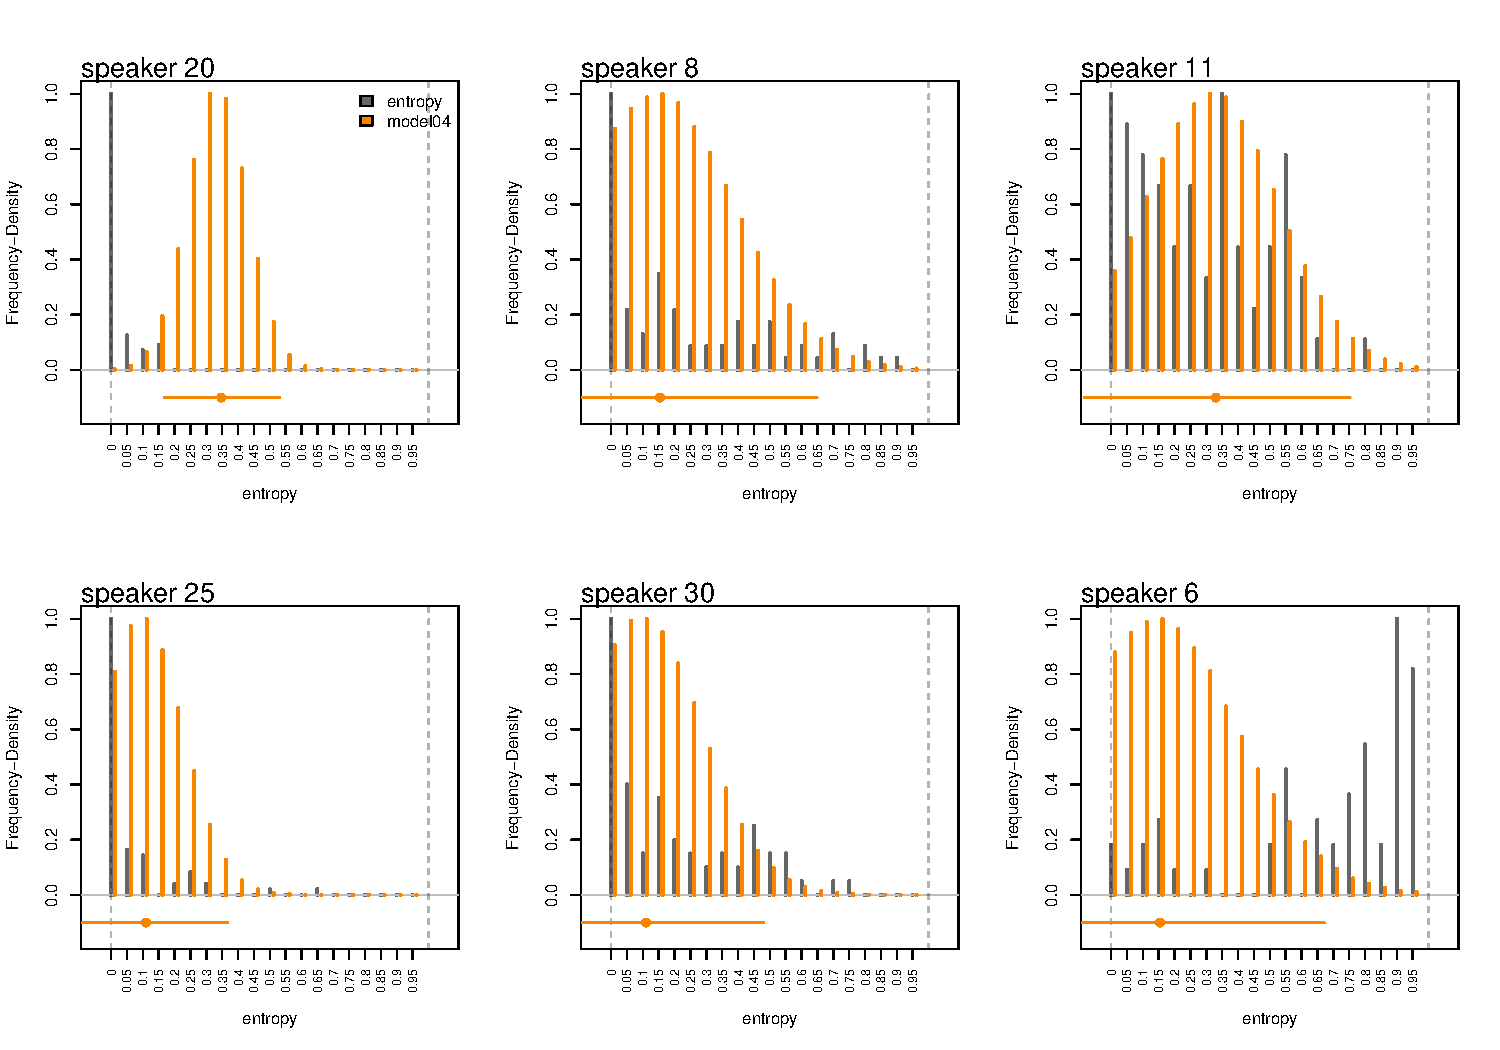
\includegraphics{index_files/figure-pdf/fig-rq1-pred-speaker_model04-1.pdf}

}

\caption{\label{fig-rq1-pred-speaker_model04}Model 4: Entropy scores
density for selected speakers. \textbf{\emph{Note:}} Black bars denote
the true data density, orange bars describe the predicted data density}

\end{figure}%

\phantomsection\label{cell-fig-rq1-pred-speaker_model10}
\begin{figure}[H]

\centering{

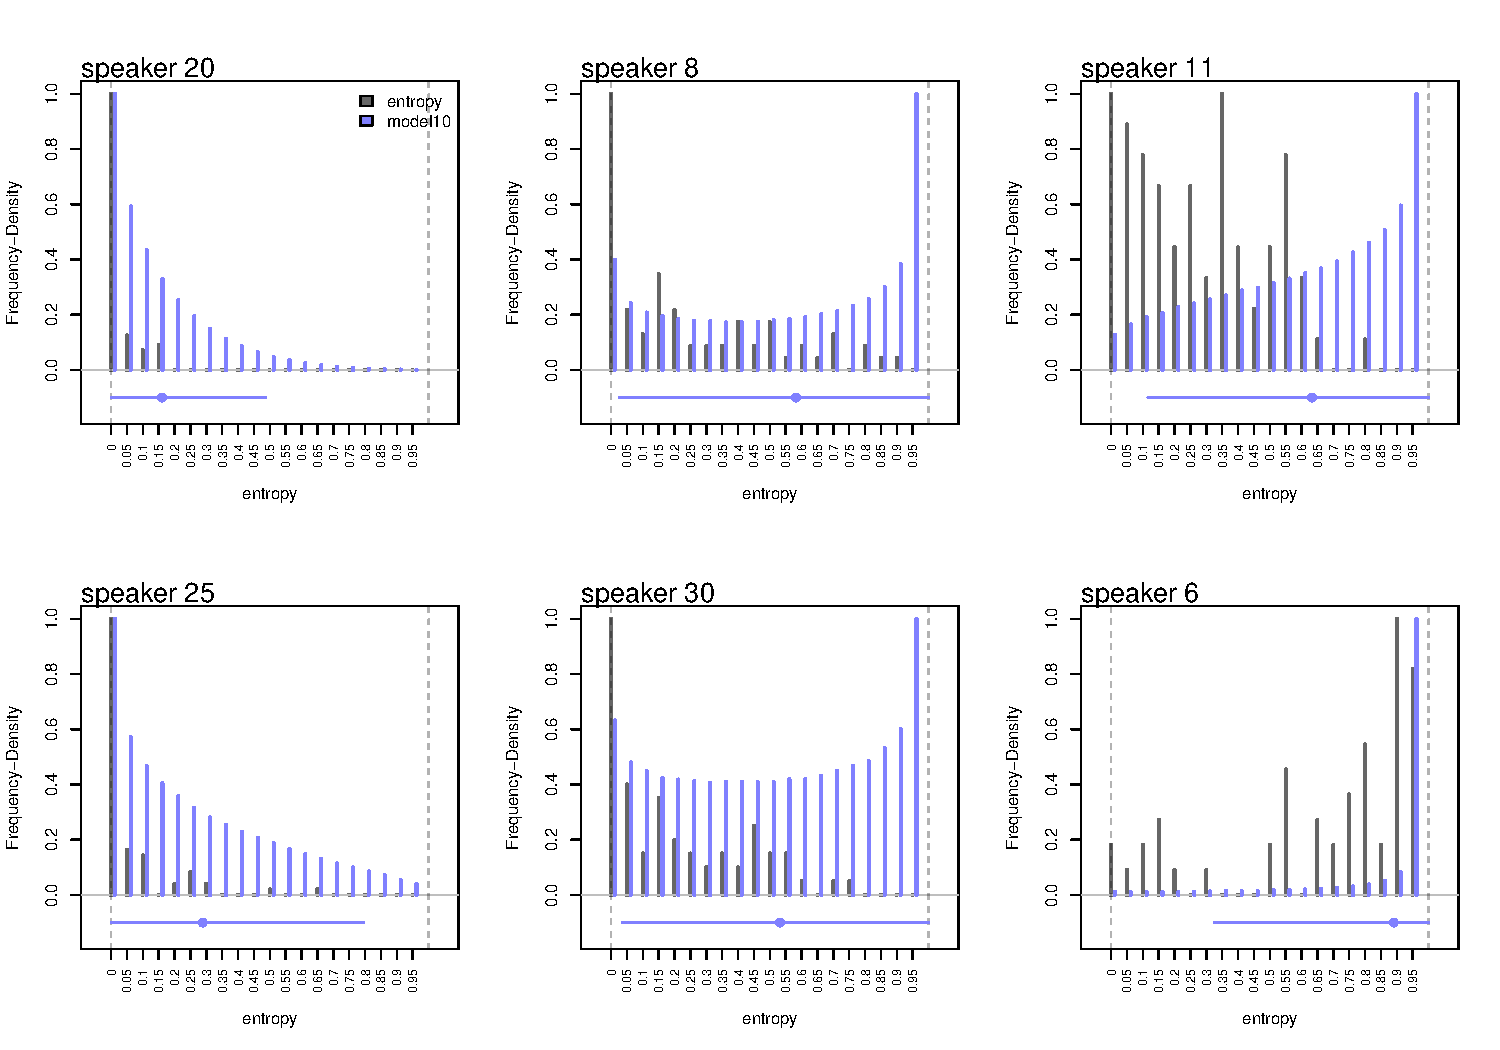
\includegraphics{index_files/figure-pdf/fig-rq1-pred-speaker_model10-1.pdf}

}

\caption{\label{fig-rq1-pred-speaker_model10}Model 10: Entropy scores
density for selected speakers. \textbf{\emph{Note:}} Black bars denote
the true data density, blue bars describe the predicted data density}

\end{figure}%

\phantomsection\label{cell-fig-rq1-model-outliers}
\begin{figure}[H]

\centering{

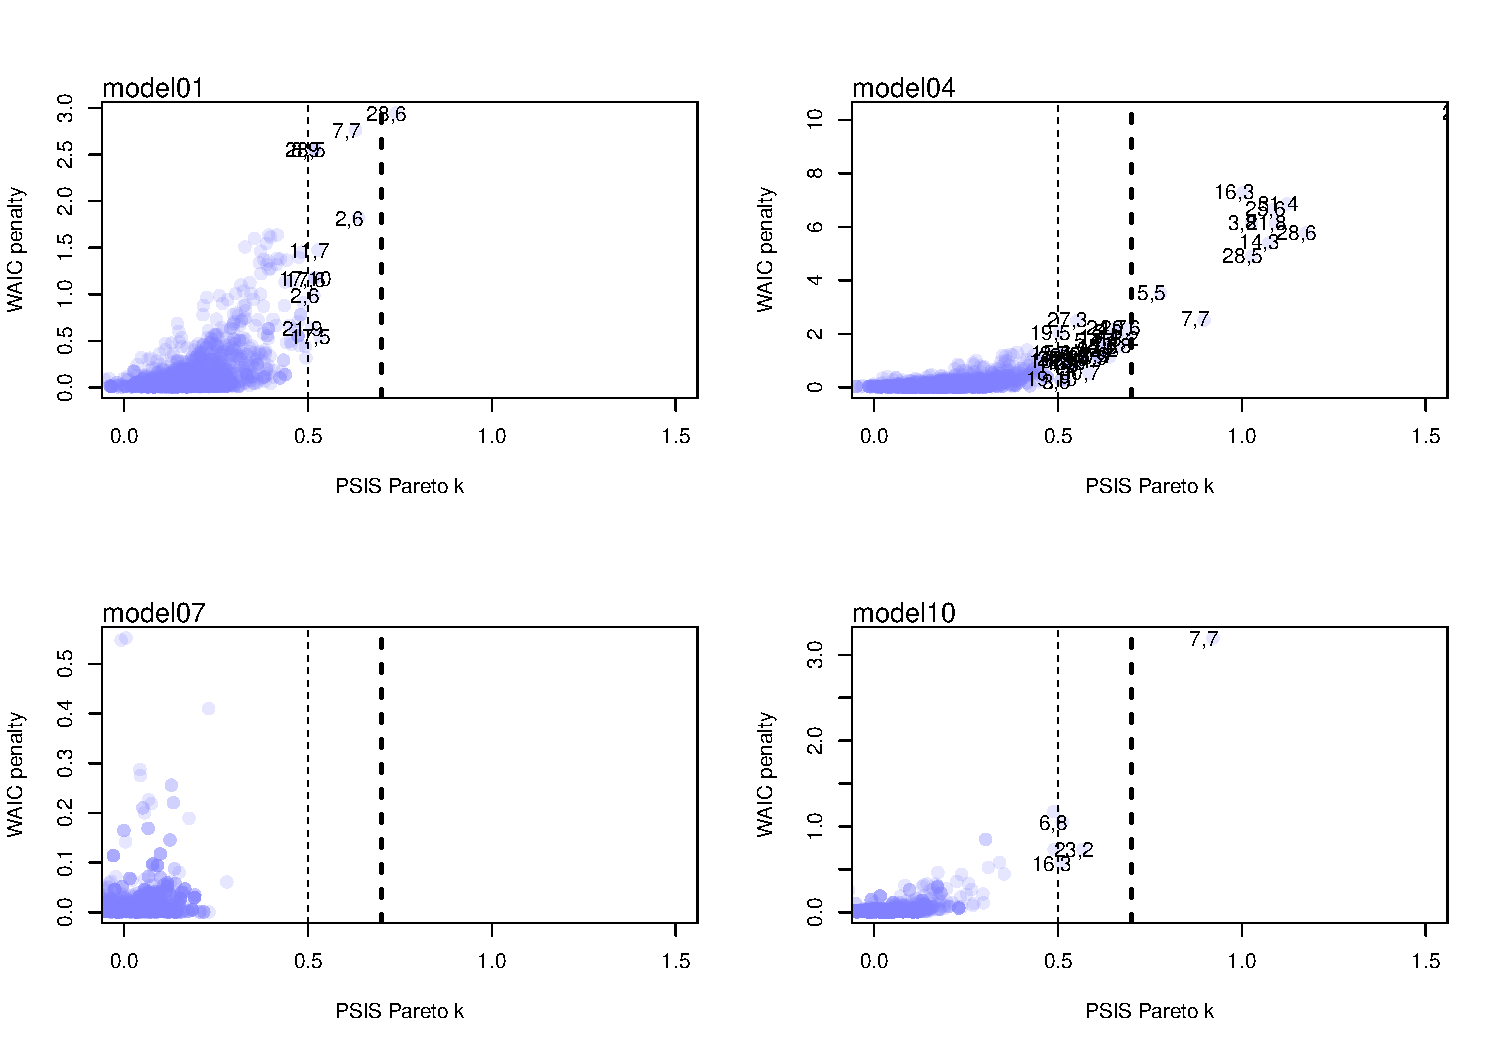
\includegraphics{index_files/figure-pdf/fig-rq1-model-outliers-1.pdf}

}

\caption{\label{fig-rq1-model-outliers}Outlier identification and
analysis for selected models. \textbf{\emph{Note:}} Thin and thick
vertical discontinuous line indicate threshold of 0.5 and 0.7,
respectively. Number pair texts indicate the observation pair of speaker
and sentence index.}

\end{figure}%

\phantomsection\label{cell-fig-rq3-pred-speaker}
\begin{figure}[H]

\centering{

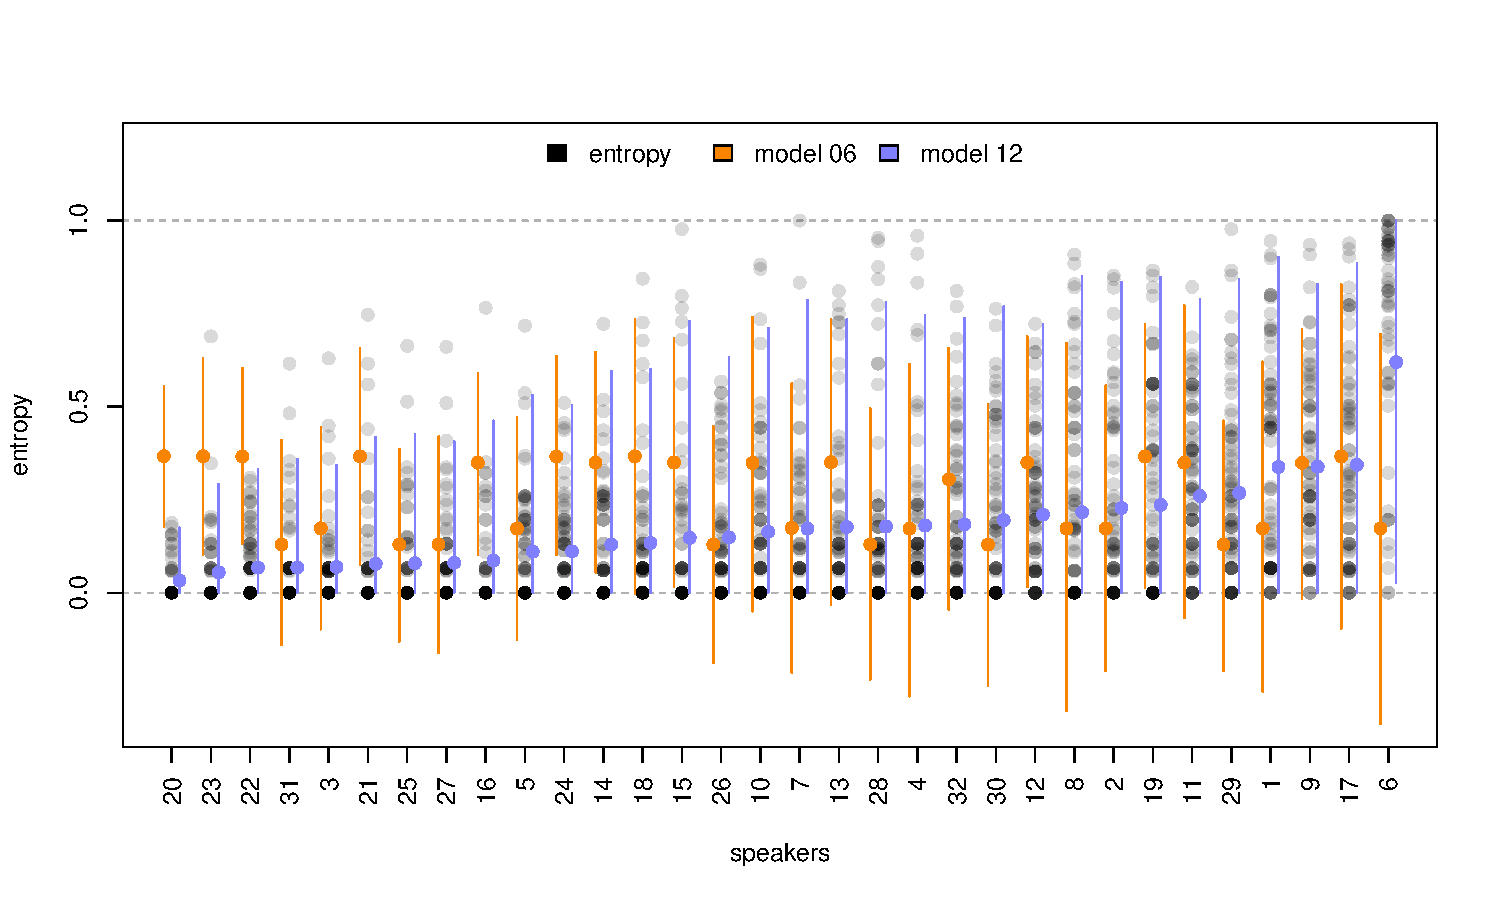
\includegraphics{index_files/figure-pdf/fig-rq3-pred-speaker-1.pdf}

}

\caption{\label{fig-rq3-pred-speaker}Entropy scores prediction for
selected models. \textcolor{blue}{\textbf{\emph{Note:}} Black points show manifest
entropy scores where darker points indicate greater overlap. Orange dots
and vertical lines show the posterior mean and 95\% HPDI derived from
Model 6. Blue dots and vertical lines show similar information from
Model 12.}}

\end{figure}%

\phantomsection\label{cell-fig-rq3-pred-speaker_model06}
\begin{figure}[H]

\centering{

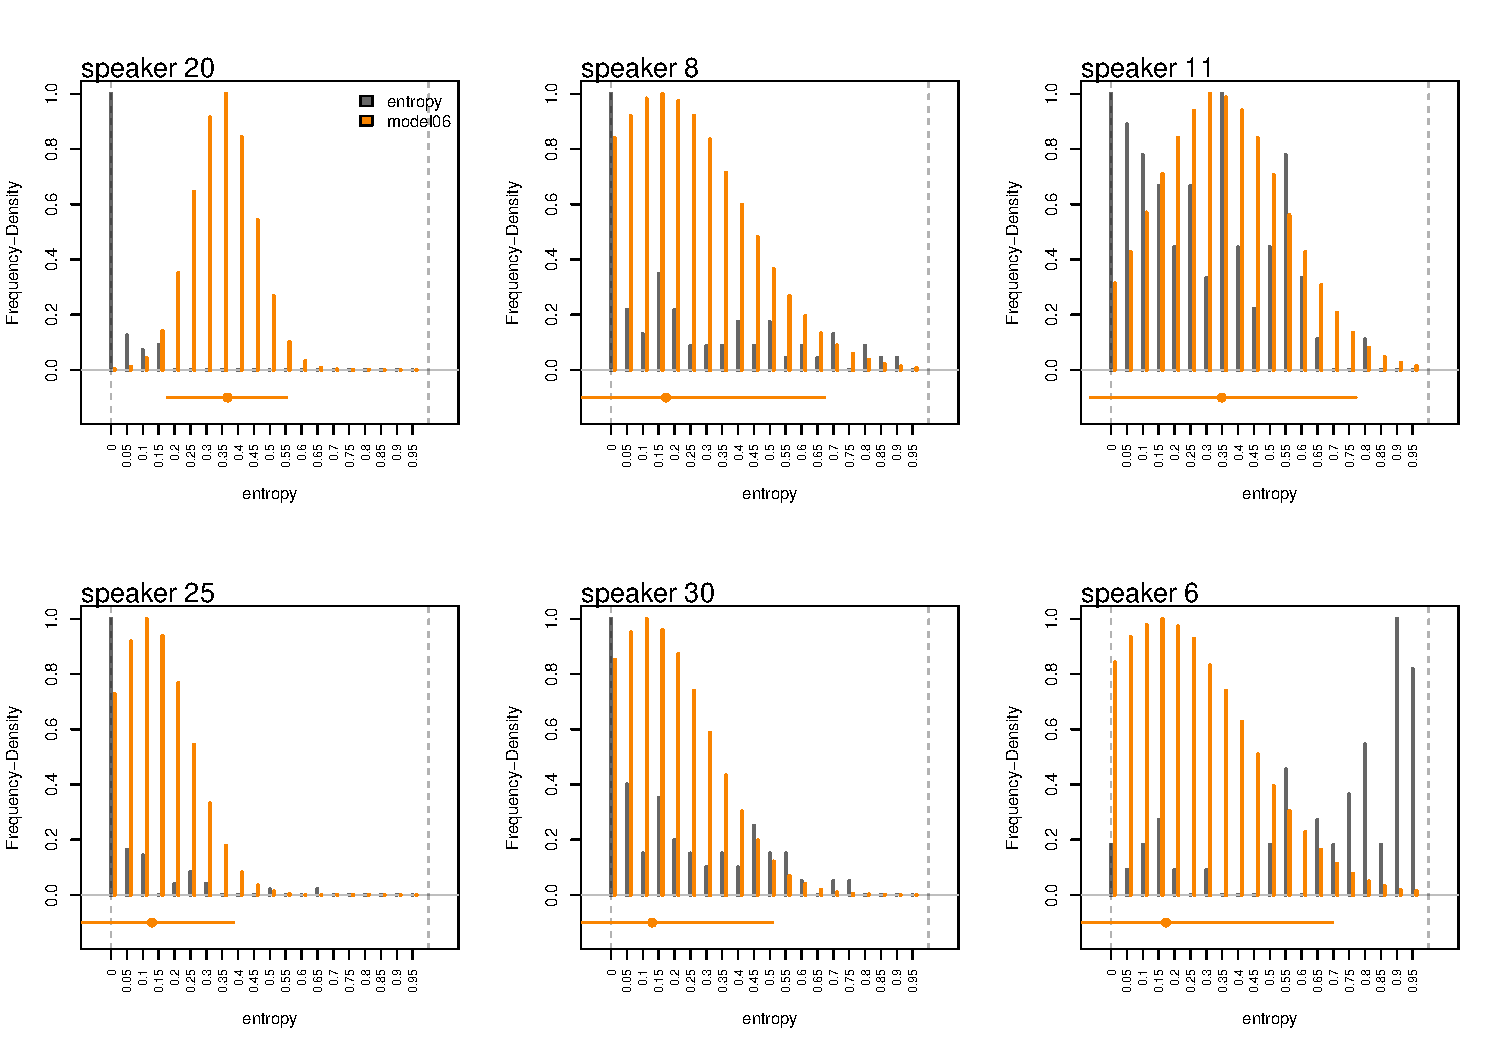
\includegraphics{index_files/figure-pdf/fig-rq3-pred-speaker_model06-1.pdf}

}

\caption{\label{fig-rq3-pred-speaker_model06}Model 6: Entropy scores
density for selected speakers. \textbf{\emph{Note:}} Black bars denote
the true data density, orange bars describe the predicted data density}

\end{figure}%

\phantomsection\label{cell-fig-rq3-pred-speaker_model12}
\begin{figure}[H]

\centering{

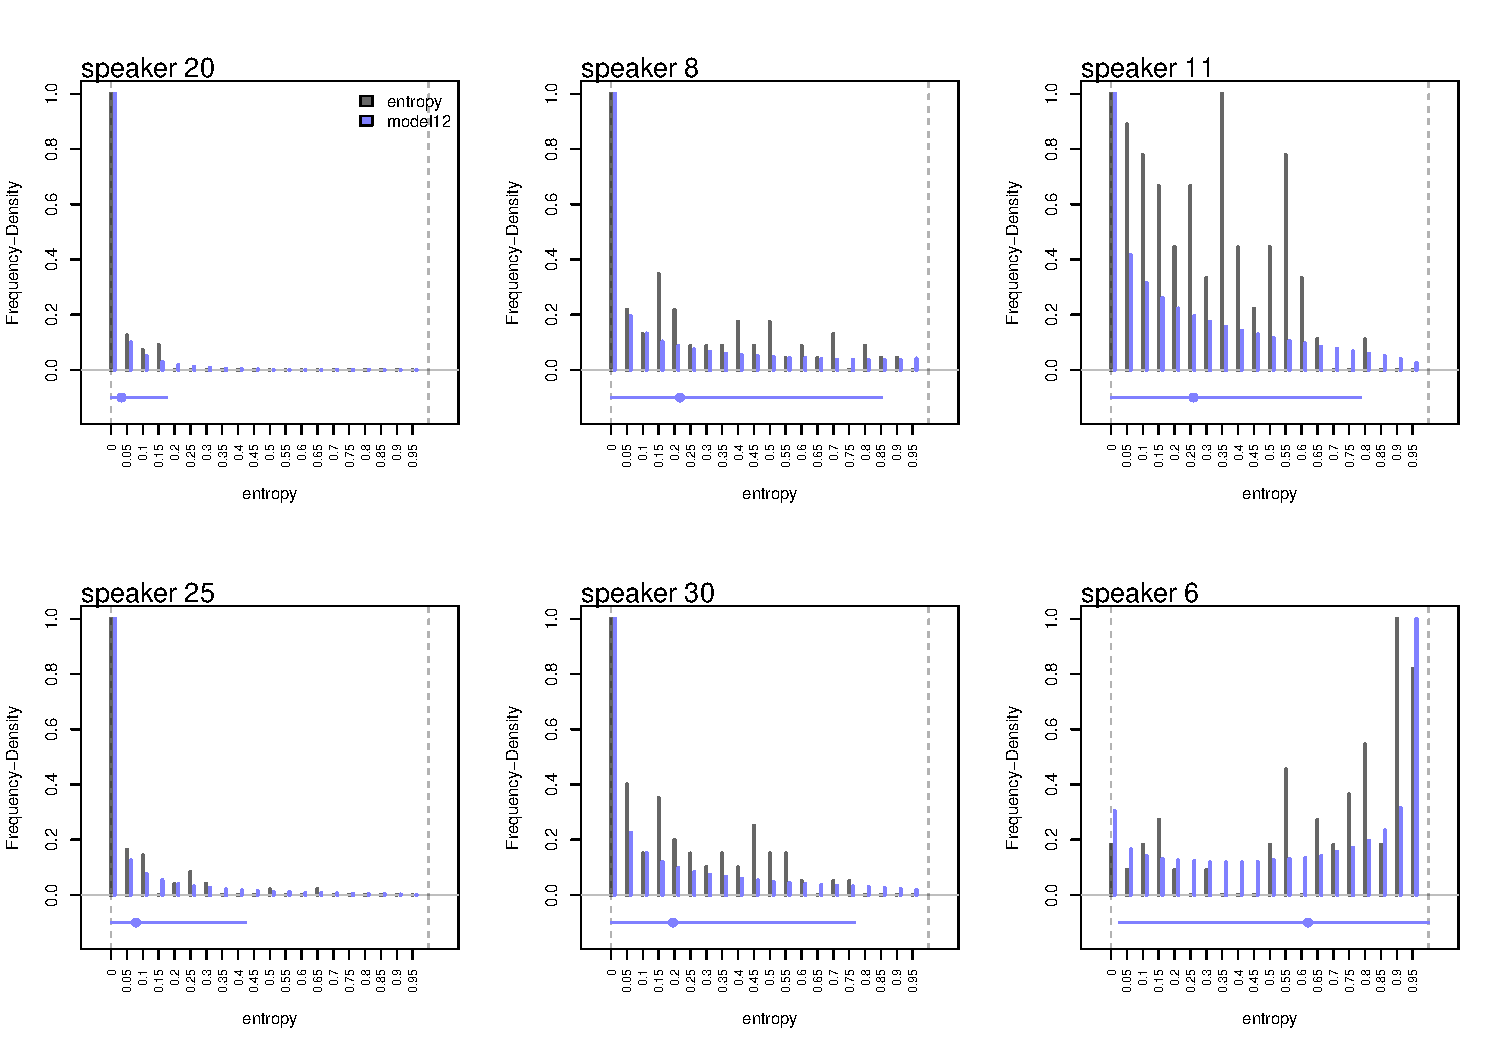
\includegraphics{index_files/figure-pdf/fig-rq3-pred-speaker_model12-1.pdf}

}

\caption{\label{fig-rq3-pred-speaker_model12}Model 12: Entropy scores
density for selected speakers. \textbf{\emph{Note:}} Black bars denote
the true data density, blue bars describe the predicted data density}

\end{figure}%

\phantomsection\label{cell-fig-rq3-model-outliers}
\begin{figure}[H]

\centering{

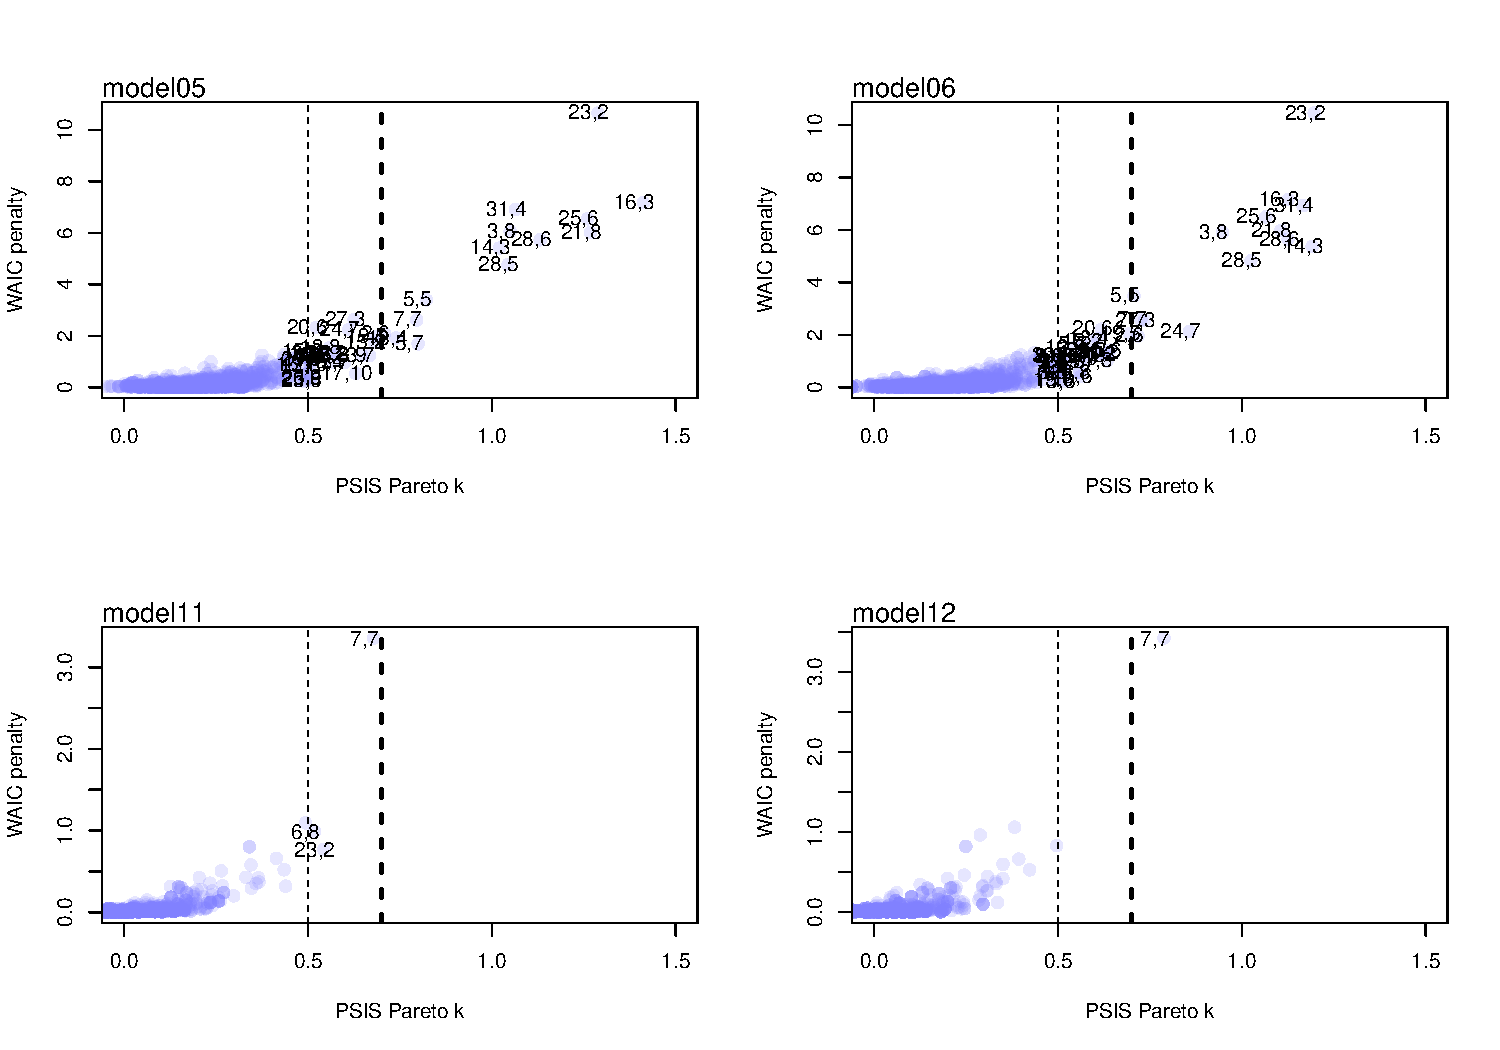
\includegraphics{index_files/figure-pdf/fig-rq3-model-outliers-1.pdf}

}

\caption{\label{fig-rq3-model-outliers}Outlier identification and
analysis for selected models. \textbf{\emph{Note:}} Thin and thick
vertical discontinuous line indicate threshold of 0.5 and 0.7,
respectively. Number pair texts indicate the observation pair of speaker
and sentence index.}

\end{figure}%

\newpage{}

\section*{References}\label{references}
\addcontentsline{toc}{section}{References}

\renewcommand{\bibsection}{}
\bibliography{references.bib}




\end{document}
